\documentclass{article}

\usepackage{graphicx} %[pdftex] OR [dvips]
\usepackage{fullpage}
\usepackage{wrapfig}
\usepackage{float}
\usepackage{titling}
\usepackage{hyperref}
\usepackage{tikz}
\usepackage{color}
\usetikzlibrary{arrows}
\usetikzlibrary{positioning}
\setlength{\droptitle}{-6em}

%!TEX root = paper/paper.tex
\usepackage{amsmath}
\usepackage{amssymb}
\usepackage{amsthm}
\usepackage{xspace}
\usepackage{color}
\usepackage{xifthen}
\usepackage{graphicx}
\usepackage{amsbsy}
\usepackage{mathtools}
\usepackage{stmaryrd}
\usepackage{url}
\usepackage{alltt}
\usepackage{varwidth}
% \usepackage{hyperref}
\usepackage{datetime}
\usepackage{subfig}
\usepackage{array}
\usepackage{multirow}
\usepackage{xargs}
\usepackage{marvosym} % for MVAt
\usepackage{bm} % for blackboard bold semicolon


%% HYPERREF COLORS
\definecolor{darkred}{rgb}{.7,0,0}
\definecolor{darkgreen}{rgb}{0,.5,0}
\definecolor{darkblue}{rgb}{0,0,.5}
% \hypersetup{
%   linktoc=page,
%   colorlinks=true,
%   linkcolor=darkred,
%   citecolor=darkgreen,
%   urlcolor=darkblue,
% }

% Coloring
\definecolor{hilite}{rgb}{0.7,0,0}
\newcommand{\hilite}[1]{\color{hilite}#1\color{black}}
\definecolor{shade}{rgb}{0.85,0.85,0.85}
\newcommand{\shade}[1]{\colorbox{shade}{\!\ensuremath{#1}\!}}

% Misc
\newcommand\evalto{\hookrightarrow}
\newcommand\elabto{\rightsquigarrow}
\newcommand\elabtox[1]{\stackrel{#1}\rightsquigarrow}
\newcommand{\yields}{\uparrow}
\newcommand\too{\Rightarrow}
\newcommand{\nil}{\cdot}
\newcommand{\eps}{\epsilon}
\newcommand{\Ups}{\Upsilon}
\newcommand{\avoids}{\mathrel{\#}}

\renewcommand{\vec}[1]{\overline{#1}}
\newcommand{\rname}[1]{\textsc{#1}}
\newcommand{\infrule}[3][]{%
  \vspace{0.5ex}
  \frac{\begin{array}{@{}c@{}}#2\end{array}}%
       {\mbox{\ensuremath{#3}}}%
  \ifthenelse{\isempty{#1}}%
             {}%
             % {\hspace{1ex}\rlap{(\rname{#1})}}%
             {\hspace{1ex}(\rname{#1})}%
  \vspace{0.5ex}
}
\newcommand{\infax}[2][]{\infrule[#1]{}{#2}}
\newcommand{\andalso}{\hspace{.5cm}}
\newcommand{\suchthat}{~\mathrm{s.t.}~}
\newenvironment{notes}%
  {\vspace{-1.5em}\begin{itemize}\setlength\itemsep{0pt}\small}%
  {\end{itemize}}
\newcommand{\macrodef}{\mathbin{\overset{\mathrm{def}}{=}}}
\newcommand{\macroiff}{\mathbin{\overset{\mathrm{def}}{\Leftrightarrow}}}


\newcommand{\ttt}[1]{\text{\tt #1}}
\newcommand{\ttul}{\texttt{\char 95}}
\newcommand{\ttcc}{\texttt{:\!:}}
\newcommand{\ttlb}{{\tt {\char '173}}}
\newcommand{\ttrb}{{\tt {\char '175}}}
\newcommand{\tsf}[1]{\textsf{#1}}

% \newcommand{\secref}[1]{\S\ref{sec:#1}}
% \newcommand{\figref}[1]{Figure~\ref{fig:#1}}
\newcommand{\marginnote}[1]{\marginpar[$\ast$ {\small #1} $\ast$]%
                                      {$\ast$ {\small #1} $\ast$}}
\newcommand{\hschange}{\marginnote{!Haskell}}
\newcommand{\TODO}{\emph{TODO}\marginnote{TODO}}
\newcommand{\parheader}[1]{\textbf{#1}\quad}

\newcommand{\file}{\ensuremath{\mathit{file}}}
\newcommand{\mapnil}{~\mathord{\not\mapsto}}

\newcommand{\Ckey}[1]{\textbf{\textsf{#1}}}
\newcommand{\Cent}[1]{\texttt{#1}}
% \newcommand{\Cmod}[1]{\texttt{[#1]}}
% \newcommand{\Csig}[1]{\texttt{[\ttcc{}#1]}}
\newcommand{\Cmod}[1]{=\texttt{[#1]}}
\newcommand{\Csig}[1]{~\ttcc{}~\texttt{[#1]}}
\newcommand{\Cpath}[1]{\ensuremath{\mathsf{#1}}}
\newcommand{\Cvar}[1]{\ensuremath{\mathsf{#1}}}
\newcommand{\Ccb}[1]{\text{\ttlb} {#1} \text{\ttrb}}
\newcommand{\Cpkg}[1]{\texttt{#1}}
\newcommand{\Cmv}[1]{\ensuremath{\langle #1 \rangle}}
\newcommand{\Cto}[2]{#1 \mapsto #2}
\newcommand{\Ctoo}[2]{\Cpath{#1} \mapsto \Cpath{#2}}
\newcommand{\Crm}[1]{#1 \mapnil}
\newcommand{\Crmm}[1]{\Cpath{#1} \mapnil}
\newcommand{\Cthin}[1]{\ensuremath{\langle \Ckey{only}~#1 \rangle}}
\newcommand{\Cthinn}[1]{\ensuremath{\langle \Ckey{only}~\Cpath{#1} \rangle}}
\newcommand{\Cinc}[1]{\Ckey{include}~{#1}}
\newcommand{\Cincc}[1]{\Ckey{include}~\Cpkg{#1}}
\newcommand{\Cshar}[2]{~\Ckey{where}~{#1} \equiv {#2}}
\newcommand{\Csharr}[2]{~\Ckey{where}~\Cpath{#1} \equiv \Cpath{#2}}
\newcommand{\Ctshar}[2]{~\Ckey{where}~{#1} \equiv {#2}}
\newcommand{\Ctsharr}[3]{~\Ckey{where}~\Cpath{#1}.\Cent{#3} \equiv \Cpath{#2}.\Cent{#3}}
\newcommand{\Cbinds}[1]{\left\{\!\begin{array}{l} #1 \end{array}\!\right\}}
\newcommand{\Cbindsp}[1]{\left(\!\begin{array}{l} #1 \end{array}\!\right)}
\newcommand{\Cpkgs}[1]{\[\begin{array}{l} #1\end{array}\]}
\newcommand{\Cpkgsl}[1]{\noindent\ensuremath{\begin{array}{@{}l} #1\end{array}}}
\newcommand{\Ccomment}[1]{\ttt{\emph{--~#1}}}
\newcommand{\Cimp}[1]{\Ckey{import}~\Cpkg{#1}}
\newcommand{\Cimpas}[2]{\Ckey{import}~\Cpkg{#1}~\Ckey{as}~\Cvar{#2}}

\newcommand{\Ctbinds}[1]{\left\{\!\vrule width 0.6pt \begin{array}{l} #1 \end{array} \vrule width 0.6pt \!\right\}}
\newcommand{\Ctbindsx}{\left\{\!\vrule width 0.6pt \; \vrule width 0.6pt \!\right\}}
\newcommand{\Ctbindsxx}{\left\{\!\vrule width 0.6pt \begin{array}{l}\!\!\!\!\\\!\!\!\!\end{array} \vrule width 0.6pt \!\right\}}
\newcommand{\Ctbindsxxx}{\left\{\!\vrule width 0.6pt \begin{array}{l}\!\!\!\!\\\!\!\!\!\\\!\!\!\!\end{array} \vrule width 0.6pt \!\right\}}


\newcommand{\Cpkgdef}[2]{%
  \ensuremath{
  \begin{array}{l}
  \Ckey{package}~\Cpkg{#1}~\Ckey{where}\\
  \hspace{1em}\begin{array}{l}
              #2
              \end{array}
  \end{array}}}
\newcommand{\Cpkgdefonly}[3]{%
  \ensuremath{
  \begin{array}{l}
  \Ckey{package}~\Cpkg{#1}\Cvar{(#2)}~\Ckey{where}\\
  \hspace{1em}\begin{array}{l}
              #3
              \end{array}
  \end{array}}}
\newcommand{\Ccc}{\mathbin{\ttcc{}}}
\newcommand{\Cbinmod}[2]{\Cvar{#1} = \texttt{[#2]}}
\newcommand{\Cbinsig}[2]{\Cvar{#1} \Ccc \texttt{[#2]}}
\newcommand{\Cinconly}[2]{\Ckey{include}~\Cpkg{#1}\Cvar{(#2)}}
\newcommand{\Cimponly}[2]{\Ckey{import}~\Cpkg{#1}\Cvar{(#2)}}
\newcommand{\Cimpmv}[3]{\Ckey{import}~\Cpkg{#1}\langle\Cvar{#2}\mapsto\Cvar{#3}\rangle}





\newcommand{\oxb}[1]{\llbracket #1 \rrbracket}
\newcommand{\coxb}[1]{\{\hspace{-.5ex}| #1 |\hspace{-.5ex}\}}
\newcommand{\coxbv}[1]{\coxb{\vec{#1}}}
\newcommand{\angb}[1]{\ensuremath{\boldsymbol\langle #1 \boldsymbol\rangle}\xspace}
\newcommand{\angbv}[1]{\angb{\vec{#1}}}
\newcommand{\aoxbl}{\ensuremath{\boldsymbol\langle\hspace{-.5ex}|}}
\newcommand{\aoxbr}{\ensuremath{|\hspace{-.5ex}\boldsymbol\rangle}\xspace}
\newcommand{\aoxb}[1]{\ensuremath{\aoxbl{#1}\aoxbr}}
\newcommand{\aoxbv}[1]{\aoxb{\vec{#1}}}
\newcommand{\poxb}[1]{\ensuremath{%
  (\hspace{-.5ex}|%
  #1%
  |\hspace{-.5ex})}\xspace}
\newcommand{\stof}[1]{{#1}^{\star}}
% \newcommand{\stof}[1]{\ensuremath{\underline{#1}}}
\newcommand{\sh}[1]{\ensuremath{\tilde{#1}}}


% \newenvironment{code}[1][t]%
%   {\ignorespaces\begin{varwidth}[#1]{\textwidth}\begin{alltt}}%
%   {\end{alltt}\end{varwidth}\ignorespacesafterend}
% \newenvironment{codel}[1][t]%
%   {\noindent\begin{varwidth}[#1]{\textwidth}\noindent\begin{alltt}}%
%   {\end{alltt}\end{varwidth}\ignorespacesafterend}


%% hack for subfloats in subfig -------------
\makeatletter
\newbox\sf@box
\newenvironment{SubFloat}[2][]%
  {\def\sf@one{#1}%
   \def\sf@two{#2}%
   \setbox\sf@box\hbox
   \bgroup}%
  {\egroup
   \ifx\@empty\sf@two\@empty\relax
     \def\sf@two{\@empty}
   \fi
   \ifx\@empty\sf@one\@empty\relax
     \subfloat[\sf@two]{\box\sf@box}%
   \else
     \subfloat[\sf@one][\sf@two]{\box\sf@box}%
   \fi}
\makeatother
%% ------------------------------------------

%% hack for top-aligned tabular cells -------------
\newsavebox\topalignbox
\newcolumntype{L}{%
  >{\begin{lrbox}\topalignbox
    \rule{0pt}{\ht\strutbox}}
  l
  <{\end{lrbox}%
    \raisebox{\dimexpr-\height+\ht\strutbox\relax}%
      {\usebox\topalignbox}}}
\newcolumntype{C}{%
  >{\begin{lrbox}\topalignbox
    \rule{0pt}{\ht\strutbox}}
  c
  <{\end{lrbox}%
    \raisebox{\dimexpr-\height+\ht\strutbox\relax}%
      {\usebox\topalignbox}}}
\newcolumntype{R}{%
  >{\begin{lrbox}\topalignbox
    \rule{0pt}{\ht\strutbox}}
  r
  <{\end{lrbox}%
    \raisebox{\dimexpr-\height+\ht\strutbox\relax}%
      {\usebox\topalignbox}}}
%% ------------------------------------------------

\newcommand\syn[1]{\textsf{#1}}
\newcommand\bsyn[1]{\textsf{\bfseries #1}}
\newcommand\msyn[1]{\textsf{#1}}
\newcommand{\cc}{\mathop{::}}

% \newcommand{\Eimp}[1]{\bsyn{import}~{#1}}
% \newcommand{\Eonly}[2]{#1~\bsyn{only}~{#2}}
% \newcommand{\Ehide}[1]{~\bsyn{hide}~{#1}}
% \newcommand{\Enew}[1]{\bsyn{new}~{#1}}
% \newcommand{\Elocal}[2]{\bsyn{local}~{#1}~\bsyn{in}~{#2}}
% \newcommand{\Smv}[3]{\Emv[]{#1}{#2}{#3}}
\newcommand{\Srm}[2]{#1 \mathord{\setminus} #2}

\newcommand{\cpath}{\varrho}
\newcommand{\fpath}{\rho}

\newcommand{\ie}{\emph{i.e.},\xspace}
\newcommand{\eg}{\emph{e.g.},~}
\newcommand{\etal}{\emph{et al.}}

\renewcommand{\P}[1]{\Cpkg{#1}}
\newcommand{\X}[1]{\Cvar{#1}}
\newcommand{\E}{\mathcal{E}}
\newcommand{\C}{\mathcal{C}}
\newcommand{\M}{\mathcal{M}}
\newcommand{\B}{\mathcal{B}}
\newcommand{\R}{\mathcal{R}}
\newcommand{\K}{\mathcal{K}}
\renewcommand{\L}{\mathcal{L}}
\newcommand{\D}{\mathcal{D}}

%%%% NEW

\newdateformat{numericdate}{%
\THEYEAR.\twodigit{\THEMONTH}.\twodigit{\THEDAY}
}

% EL DEFNS
\newcommand{\shal}[1]{\syn{shallow}(#1)}
\newcommand{\exports}[1]{\syn{exports}(#1)}
\newcommand{\Slocals}[1]{\syn{locals}(#1)}
\newcommand{\Slocalsi}[2]{\syn{locals}(#1; #2)}
\newcommand{\specs}[1]{\syn{specs}(#1)}
\newcommand{\ELmkespc}[2]{\syn{mkespc}(#1;#2)}
\newcommand{\Smkeenv}[1]{\syn{mkeenv}(#1)}
\newcommand{\Smklocaleenv}[2]{\syn{mklocaleenv}(#1;#2)}
\newcommand{\Smklocaleenvespcs}[1]{\syn{mklocaleenv}(#1)}
\newcommand{\Smkphnms}[1]{\syn{mkphnms}(#1)}
\newcommand{\Smkphnm}[1]{\syn{mkphnm}(#1)}
\newcommand{\Sfilterespc}[2]{\syn{filterespc}(#1;#2)}
\newcommand{\Sfilterespcs}[2]{\syn{filterespcs}(#1;#2)}
\newcommand{\Simps}[1]{\syn{imps}(#1)}



% IL DEFNS
\newcommand{\dexp}{\mathit{dexp}}
\newcommand{\fexp}{\mathit{fexp}}
\newcommand{\tfexp}{\mathit{tfexp}}
\newcommand{\pexp}{\mathit{pexp}}
\newcommand{\dtyp}{\mathit{dtyp}}
\newcommand{\ftyp}{\mathit{ftyp}}
\newcommand{\hsmod}{\mathit{hsmod}}
\newcommand{\fenv}{\mathit{fenv}}
\newcommand{\ILmkmod}[6]{\syn{mkmod}(#1; #2; #3; #4; #5; #6)}
\newcommand{\ILmkstubs}[3]{\syn{mkstubs}(#1; #2; #3)}
\newcommand{\Smkstubs}[1]{\syn{mkstubs}(#1)}
\newcommand{\ILentnames}[1]{\syn{entnames}(#1)}
\newcommand{\ILmkfenv}[1]{\syn{mkfenv}(#1)}
\newcommand{\ILmkdtyp}[1]{\syn{mkdtyp}(#1)}
\newcommand{\ILmkknd}[1]{\syn{mkknd}(#1)}
\newcommand{\ILmkimpdecl}[2]{\syn{mkimpdecl}(#1;#2)}
\newcommand{\ILmkimpdecls}[2]{\syn{mkimpdecls}(#1;#2)}
\newcommand{\ILmkimpspec}[3]{\syn{mkimpspec}(#1;#2;#3)}
\newcommand{\ILmkentimp}[3]{\syn{mkentimp}(#1;#2;#3)}
\newcommand{\ILmkentimpp}[1]{\syn{mkentimp}(#1)}
\newcommand{\ILmkexp}[2]{\syn{mkexp}(#1;#2)}
\newcommand{\ILmkexpdecl}[2]{\syn{mkexpdecl}(#1;#2)}
\newcommand{\ILmkespc}[2]{\syn{mkespc}(#1;#2)}
\newcommand{\ILshal}[1]{\syn{shallow}(#1)}
\newcommand{\ILexports}[1]{\syn{exports}(#1)}
\newcommand{\ILdefns}[1]{\syn{defns}(#1)}
\newcommand{\ILdefnsi}[2]{\syn{defns}(#1;#2)}

% CORE DEFNS
\newcommand{\Hentref}{\mathit{eref}}
\newcommand{\Hentimp}{\mathit{import}}
\newcommand{\Hentexp}{\mathit{export}}
\newcommand{\Himp}{\mathit{impdecl}}
\newcommand{\Himpspec}{\mathit{impspec}}
\newcommand{\Himps}{\mathit{impdecls}}
\newcommand{\Hexps}{\mathit{expdecl}}
\newcommand{\Hdef}{\mathit{def}}
\newcommand{\Hdefs}{\mathit{defs}}
\newcommand{\Hdecl}{\mathit{decl}}
\newcommand{\Hdecls}{\mathit{decls}}
\newcommand{\Heenv}{\mathit{eenv}}
\newcommand{\Haenv}{\mathit{aenv}}
% \newcommand{\HIL}[1]{{\scriptstyle\downarrow}#1}
\newcommand{\HIL}[1]{\check{#1}}

\newcommand{\Hcmp}{\sqsubseteq}

\newcommand{\uexp}{\mathit{uexp}}
\newcommand{\utyp}{\mathit{utyp}}
\newcommand{\typ}{\mathit{typ}}
\newcommand{\knd}{\mathit{knd}}
\newcommand{\kndstar}{\ttt{*}}
\newcommand{\kndarr}[2]{#1\ensuremath{\mathbin{\ttt{->}}}#2}
\newcommand{\kenv}{\mathit{kenv}}
\newcommand{\phnm}{\mathit{phnm}}
\newcommand{\spc}{\mathit{dspc}}
\newcommand{\spcs}{\mathit{dspcs}}
\newcommand{\espc}{\mathit{espc}}
\newcommand{\espcs}{\mathit{espcs}}
\newcommand{\ds}{\mathit{ds}}

\newcommand{\shctx}{\sh{\Xi}_{\syn{ctx}}}
\newcommand{\shctxsigma}{\sh{\Sigma}_{\syn{ctx}}}

\newcommand{\vdashsh}{\Vdash}

% \newcommand{\vdashghc}{\vdash_{\!\!\mathrm{c}}^{\!\!\mathrm{\scriptscriptstyle EL}}}
% \newcommand{\vdashghcil}{\vdash_{\!\!\mathrm{c}}^{\!\!\mathrm{\scriptscriptstyle IL}}}
% \newcommand{\vdashshghc}{\vdashsh_{\!\!\mathrm{c}}^{\!\!\mathrm{\scriptscriptstyle EL}}}
\newcommand{\vdashghc}{\vdash_{\!\!\mathrm{c}}}
\newcommand{\vdashghcil}{\vdash_{\!\!\mathrm{c}}^{\!\!\mathrm{\scriptscriptstyle IL}}}
\newcommand{\vdashshghc}{\vdashsh_{\!\!\mathrm{c}}}

% CORE STUFF
\newcommandx*{\JCModImp}[5][1=\sh\B, 2=\nu_0, usedefault=@]%
  {#1;#2 \vdashshghc #3;#4 \elabto #5}
\newcommandx*{\JIlCModImp}[5][1=\fenv, 2=f_0, usedefault=@]%
  {#1;#2 \vdashghcil #3;#4 \elabto #5}
\newcommandx*{\JCSigImp}[5][1=\sh\B, 2=\sh\tau, usedefault=@]%
  {#1;#2 \vdashshghc #3;#4 \elabto #5}

\newcommandx*{\JCImpDecl}[3][1=\sh\B, usedefault=@]%
  {#1 \vdashshghc #2 \elabto #3}
\newcommandx*{\JCImp}[4][1=\sh\B, 2=p, usedefault=@]%
  {#1;#2 \vdashshghc #3 \elabto #4}
\newcommandx*{\JIlCImpDecl}[3][1=\fenv, usedefault=@]%
  {#1 \vdashghcil #2 \elabto #3}
\newcommandx*{\JIlCImp}[4][1=\fenv, 2=f, usedefault=@]%
  {#1;#2 \vdashghcil #3 \elabto #4}

\newcommandx*{\JCModExp}[4][1=\nu_0, 2=\Heenv, usedefault=@]%
  {#1;#2 \vdashshghc #3 \elabto #4}
\newcommandx*{\JIlCModExp}[4][1=f_0, 2=\HIL\Heenv, usedefault=@]%
  {#1;#2 \vdashghcil #3 \elabto #4}

\newcommandx*{\JCModDef}[5][1=\Psi, 2=\nu_0, 3=\Heenv, usedefault=@]%
  {#1; #2; #3 \vdashghcil #4 : #5}
\newcommandx*{\JIlCModDef}[5][1=\fenv, 2=f_0, 3=\HIL\Heenv, usedefault=@]%
  {#1; #2; #3 \vdashghcil #4 : #5}
\newcommandx*{\JCSigDecl}[5][1=\Psi, 2=\sh\tau, 3=\Heenv, usedefault=@]%
  {#1; #2; #3 \vdashghcil #4 : #5}

\newcommandx*{\JCExp}[6][1=\sh\Psi, 2=\nu_0, 3=\Hdefs, 4=\Heenv, usedefault=@]%
  {#1;#2;#3;#4 \vdashshghc #5 \elabto #6}
\newcommandx*{\JIlCExp}[4][1=f_0, 2=\HIL\Heenv, usedefault=@]%
  {#1;#2 \vdashghcil #3 \elabto #4}

\newcommandx*{\JCRefExp}[7][1=\sh\Psi, 2=\nu_0, 3=\Hdefs, 4=\Heenv, usedefault=@]%
  {#1;#2;#3;#4 \vdashshghc #5 \elabto #6:#7}
\newcommandx*{\JIlCRefExp}[7][1=\fenv, 2=f_0, 3=\HIL\Hdefs, 4=\HIL\Heenv, usedefault=@]%
  {#1;#2;#3;#4 \vdashghcil #5 \elabto #6:#7}

\newcommandx*{\JCMod}[4][1=\Gamma, 2=\nu_0, usedefault=@]%
  {#1; #2 \vdashghc #3 : #4}
\newcommandx*{\JIlCMod}[3][1=\fenv, usedefault=@]%
  {#1 \vdashghcil #2 : #3}
\newcommandx*{\JCSig}[5][1=\Gamma, 2=\sh\tau, usedefault=@]%
  {#1; #2 \vdashghc #3 \elabto #4;#5}
\newcommandx*{\JCShSig}[5][1=\Gamma, 2=\sh\tau, usedefault=@]%
  {#1; #2 \vdashghc #3 \elabto #4;#5}
\newcommandx*{\JCModElab}[5][1=\Gamma, 2=\nu_0, usedefault=@]%
  % {#1; #2 \vdashghc #3 : #4 \elabto #5}
  {#1; #2 \vdashghc #3 : #4 \;\shade{\elabto #5}}

\newcommandx*{\JCWfEenv}[2][1=\Haenv, usedefault=@]%
  {#1 \vdashshghc #2~\syn{wf}}
\newcommandx*{\JCWfEenvMap}[2][1=\Haenv, usedefault=@]%
  {#1 \vdashshghc #2~\syn{wf}}
\newcommandx*{\JIlCWfEenv}[2][1=\HIL\Haenv, usedefault=@]%
  {#1 \vdashghcil #2~\syn{wf}}
\newcommandx*{\JIlCWfEenvMap}[2][1=\HIL\Haenv, usedefault=@]%
  {#1 \vdashghcil #2~\syn{wf}}

\newcommandx*{\JIlTfexp}[3][1=\fenv, 2=f_0, usedefault=@]%
  {#1; #2 \vdash #3}



  % IL STUFF

\newcommandx*{\JIlWf}[2][1=\fenv, usedefault=@]%
  {#1 \vdash #2 ~\syn{wf}}
\newcommandx*{\JIlKnd}[4][1=\fenv, 2=\kenv, usedefault=@]%
  {#1;#2 \vdashghcil #3 \mathrel{\cc} #4}
% \newcommandx*{\JIlSub}[4][1=\fenv, 2=f, usedefault=@]%
%   {#1;#2 \vdash #3 \le #4}
\newcommandx*{\JIlSub}[2][usedefault=@]%
  {\vdash #1 \le #2}
\newcommandx*{\JIlMerge}[3][usedefault=@]%
  {\vdash #1 \oplus #2 \Rightarrow #3}

\newcommandx*{\JIlDexp}[2][1=\fenv, usedefault=@]%
  {#1 \vdash #2}
\newcommandx*{\JIlDexpTyp}[3][1=\fenv, usedefault=@]%
  {#1 \vdash #2 : #3}

\newcommandx*{\JIlWfFenv}[2][1=\nil, usedefault=@]%
  {#1 \vdash #2 ~\syn{wf}}
\newcommandx*{\JIlWfFtyp}[2][1=\fenv, usedefault=@]%
  {#1 \vdash #2 ~\syn{wf}}
\newcommandx*{\JIlWfSpc}[2][1=\fenv, usedefault=@]%
  {#1 \vdash #2 ~\syn{wf}}
\newcommandx*{\JIlWfESpc}[2][1=\fenv, usedefault=@]%
  {#1 \vdash #2 ~\syn{wf}}
\newcommandx*{\JIlWfSig}[2][1=\fenv, usedefault=@]%
  {#1 \vdash #2 ~\syn{wf}}
\newcommandx*{\JIlWfFtypSpecs}[2][1=\fenv, usedefault=@]%
  {#1 \vdash #2 ~\syn{specs-wf}}
\newcommandx*{\JIlWfFtypExps}[2][1=\fenv, usedefault=@]%
  {#1 \vdash #2 ~\syn{exports-wf}}
\newcommandx*{\JIlWfFenvDeps}[2][1=\fenv, usedefault=@]%
  {#1 \vdash #2 ~\syn{deps-wf}}

% WF TYPE STUFF IN EL
\newcommandx*{\JPkgValid}[1]%
  {\vdash #1 ~\syn{pkg-valid}}
\newcommandx*{\JWfPkgCtx}[1][1=\Delta, usedefault=@]%
  {\vdash #1 ~\syn{wf}}
\newcommandx*{\JWfPhCtx}[2][1=\nil, usedefault=@]%
  {#1 \vdash #2 ~\syn{wf}}
\newcommandx*{\JWfModTyp}[2][1=\Psi, usedefault=@]%
  {#1 \vdash #2 ~\syn{wf}}
\newcommandx*{\JWfModTypPol}[3][1=\Psi, usedefault=@]%
  {#1 \vdash #2^{#3} ~\syn{wf}}
\newcommandx*{\JWfLogSig}[2][1=\Psi, usedefault=@]%
  {#1 \vdash #2 ~\syn{wf}}
\newcommandx*{\JWfSpc}[2][1=\Psi, usedefault=@]%
  {#1 \vdash #2 ~\syn{wf}}
\newcommandx*{\JWfESpc}[2][1=\Psi, usedefault=@]%
  {#1 \vdash #2 ~\syn{wf}}
\newcommandx*{\JWfSig}[2][1=\nil, usedefault=@]%
  {#1 \vdash #2 ~\syn{wf}}
\newcommandx*{\JWfModTypSpecs}[2][1=\Psi, usedefault=@]%
  {#1 \vdash #2 ~\syn{specs-wf}}
\newcommandx*{\JWfModTypPolSpecs}[3][1=\Psi, usedefault=@]%
  {#1 \vdash #2^{#3} ~\syn{specs-wf}}
\newcommandx*{\JWfModTypExps}[2][1=\Psi, usedefault=@]%
  {#1 \vdash #2 ~\syn{exports-wf}}
\newcommandx*{\JWfPhCtxDeps}[2][1=\Psi, usedefault=@]%
  {#1 \vdash #2 ~\syn{deps-wf}}
\newcommandx*{\JWfPhCtxDepsOne}[4][1=\Psi, usedefault=@]%
  {#1 \vdash \styp{#2}{#3}{#4} ~\syn{deps-wf}}

% WF SHAPE STUFF IN EL
\newcommandx*{\JWfShPhCtx}[2][1=\nil, usedefault=@]%
  {#1 \vdashsh #2 ~\syn{wf}}
\newcommandx*{\JWfModSh}[2][1=\sh\Psi, usedefault=@]%
  {#1 \vdashsh #2 ~\syn{wf}}
\newcommandx*{\JWfModShPol}[3][1=\sh\Psi, usedefault=@]%
  {#1 \vdashsh #2^{#3} ~\syn{wf}}
\newcommandx*{\JWfShLogSig}[2][1=\sh\Psi, usedefault=@]%
  {#1 \vdashsh #2 ~\syn{wf}}
\newcommandx*{\JWfShSpc}[2][1=\sh\Psi, usedefault=@]%
  {#1 \vdashsh #2 ~\syn{wf}}
\newcommandx*{\JWfShESpc}[2][1=\sh\Psi, usedefault=@]%
  {#1 \vdashsh #2 ~\syn{wf}}
\newcommandx*{\JWfShSig}[2][1=\nil, usedefault=@]%
  {#1 \vdashsh #2 ~\syn{wf}}
\newcommandx*{\JWfModShSpecs}[2][1=\sh\Psi, usedefault=@]%
  {#1 \vdashsh #2 ~\syn{specs-wf}}
\newcommandx*{\JWfModShPolSpecs}[3][1=\sh\Psi, usedefault=@]%
  {#1 \vdashsh #2^{#3} ~\syn{specs-wf}}
\newcommandx*{\JWfModShExps}[2][1=\sh\Psi, usedefault=@]%
  {#1 \vdashsh #2 ~\syn{exports-wf}}
\newcommandx*{\JWfEenv}[4][1=\sh\Psi, 2=\nu_0, 3=\Hdefs, usedefault=@]%
  {#1;#2;#3 \vdashshghc #4 ~\syn{wf}}

\newcommandx*{\JCoreKnd}[4][1=\Psi, 2=\kenv, usedefault=@]%
  {#1;#2 \vdashghc #3 \mathrel{\cc} #4}

\newcommandx*{\JStampEq}[2]%
  {\vdash #1 \equiv #2}
\newcommandx*{\JStampNeq}[2]%
  {\vdash #1 \not\equiv #2}
\newcommandx*{\JUnif}[3]%
  {\syn{unify}(#1 \doteq #2) \elabto #3}
\newcommandx*{\JUnifM}[2]%
  {\syn{unify}(#1) \elabto #2}

\newcommandx*{\JModTypWf}[1]%
  {\vdash #1 ~\syn{wf}}
  
\newcommandx*{\JModSub}[2]%
  {\vdash #1 \le #2}
\newcommandx*{\JModSup}[2]%
  {\vdash #1 \ge #2}
\newcommandx*{\JShModSub}[2]%
  {\vdashsh #1 \le #2}

\newcommandx*{\JModEq}[2]%
  {\vdash #1 \equiv #2}
% \newcommandx*{\JCShModEq}[3][3=\C]%
%   {\vdashsh #1 \equiv #2 \mathbin{|} #3}

\newcommandx*{\JETyp}[4][1=\Gamma, 2=\shctxsigma, usedefault=@]%
  {#1;#2 \vdash #3 : #4}
\newcommandx*{\JETypElab}[5][1=\Gamma, 2=\shctxsigma, usedefault=@]%
  {\JETyp[#1][#2]{#3}{#4} \elabto #5}
\newcommandx*{\JESh}[3][1=\sh\Gamma, usedefault=@]%
  {#1 \vdashsh #2 \Rightarrow #3}

\newcommandx*{\JBTyp}[5][1=\Delta, 2=\Gamma, 3=\shctx, usedefault=@]%
  {#1;#2;#3 \vdash #4 : #5}
\newcommandx*{\JBTypElab}[6][1=\Delta, 2=\Gamma, 3=\shctx, usedefault=@]%
  % {\JBTyp[#1][#2][#3]{#4}{#5} \elabto #6}
  {\JBTyp[#1][#2][#3]{#4}{#5} \;\shade{\elabto #6}}
\newcommandx*{\JBSh}[4][1=\Delta, 2=\sh\Gamma, usedefault=@]%
  {#1;#2 \vdashsh #3 \Rightarrow #4}
  
\newcommandx*{\JBVTyp}[4][1=\Delta, 2=\shctx, usedefault=@]%
  {#1;#2 \vdash #3 : #4}
\newcommandx*{\JBVTypElab}[5][1=\Delta, 2=\shctx, usedefault=@]%
  % {\JBVTyp[#1][#2]{#3}{#4} \elabto #5}
  {\JBVTyp[#1][#2]{#3}{#4} \;\shade{\elabto #5}}
\newcommandx*{\JBVSh}[4][1=\Delta, usedefault=@]%
  {#1 \vdashsh #2 \Rightarrow #3;\, #4}
  
\newcommandx*{\JImp}[3][1=\Gamma, usedefault=@]%
  {#1 \vdashimp #2 \elabto #3}
\newcommandx*{\JShImp}[3][1=\sh\Gamma, usedefault=@]%
  {#1 \vdashshimp #2 \elabto #3}
  
\newcommandx*{\JGhcMod}[4]%
  {#1; #2 \vdashghc #3 : #4}
\newcommandx*{\JShGhcMod}[4]%
  {#1; #2 \vdashshghc #3 : #4}
  
\newcommandx*{\JGhcSig}[5]%
  {#1; #2 \vdashghc #3 \elabto #4;#5}
\newcommandx*{\JShGhcSig}[5]%
  {#1; #2 \vdashshghc #3 \elabto #4;#5}
  
\newcommandx*{\JThin}[3][1=t, usedefault=@]%
  {\vdash #2 \xrightarrow{~#1~} #3}
\newcommandx*{\JShThin}[3][1=t, usedefault=@]%
  {\vdashsh #2 \xrightarrow{~#1~} #3}

\newcommandx*{\JShMatch}[3][1=\nu, usedefault=@]%
  {#1 \vdash #2 \sqsubseteq #3}
  
\newcommandx*{\JShTrans}[4]%
  {\vdash #1 \le_{#2} #3 \elabto #4}
  
\newcommandx*{\JMerge}[3]%
  {\vdash #1 + #2 \Rightarrow #3}
\newcommandx*{\JShMerge}[5]%
  {\vdashsh #1 + #2 \Rightarrow #3;\, #4;\, #5}
\newcommandx*{\JShMergeNew}[4]%
  {\vdashsh #1 + #2 \Rightarrow #3;\, #4}
\newcommandx*{\JShMergeSimple}[3]%
  {\vdashsh #1 + #2 \Rightarrow #3}

\newcommandx*{\JDTyp}[3][1=\Delta, usedefault=@]%
  {#1 \vdash #2 : #3}
\newcommandx*{\JDTypElab}[4][1=\Delta, usedefault=@]%
  % {#1 \vdash #2 : #3 \elabto #4}
  {#1 \vdash #2 : #3 \;\shade{\elabto #4}}

\newcommandx*{\JTTyp}[2][1=\Delta, usedefault=@]%
  {#1 \vdash #2}

\newcommandx*{\JSound}[3][1=\Psi_\syn{ctx}, usedefault=@]%
  {#1 \vdash #2 \sim #3}

\newcommandx*{\JSoundOne}[4][1=\Psi, 2=\fenv, usedefault=@]%
  {\vdash #3 \sim #4}
% \newcommand{\Smodi}[4]{\ensuremath{\oxb{=#2 \cc #3 \imps #4}^{#1}}}
\newcommand{\Smodi}[3]{\ensuremath{\oxb{=#2 \cc #3}^{#1}}}
\newcommand{\Smod}[2]{\Smodi{+}{#1}{#2}}
\newcommand{\Ssig}[2]{\Smodi{-}{#1}{#2}}
\newcommand{\Sreq}[2]{\Smodi{?}{#1}{#2}}
\newcommand{\Shole}[2]{\Smodi{\circ}{#1}{#2}}

\newcommand{\SSmodi}[2]{\ensuremath{\oxb{=#2}^{#1}}}
\newcommand{\SSmod}[1]{\SSmodi{+}{#1}}
\newcommand{\SSsig}[1]{\SSmodi{-}{#1}}
\newcommand{\SSreq}[1]{\SSmodi{?}{#1}}
\newcommand{\SShole}[1]{\SSmodi{\circ}{#1}}

% \newcommand{\styp}[3]{\oxb{{#1}\cc{#2}}^{#3}}
\newcommand{\styp}[3]{{#1}{:}{#2}^{#3}}
\newcommand{\stm}[2]{\styp{#1}{#2}{\scriptscriptstyle+}}
\newcommand{\sts}[2]{\styp{#1}{#2}{\scriptscriptstyle-}}

% \newcommand{\mtypsep}{[\!]}
\newcommand{\mtypsep}{\mbox{$\bm{;}$}}
\newcommand{\mtypsepsp}{\hspace{.3em}}
\newcommand{\msh}[3]{\aoxb{#1 ~\mtypsep~ #2 ~\mtypsep~ #3}}
\newcommand{\mtyp}[3]{
  \aoxb{\mtypsepsp #1 \mtypsepsp\mtypsep\mtypsepsp
        #2 \mtypsepsp\mtypsep\mtypsepsp
        #3 \mtypsepsp}}
\newcommand{\bigmtyp}[3]{\ensuremath{
  \left\langle\!\vrule \begin{array}{l}
    #1 ~\mtypsep \\[0pt]
    #2 ~\mtypsep \\
    #3
  \end{array} \vrule\!\right\rangle
}}


\newcommand{\mtypm}[2]{\mtyp{#1}{#2}^{\scriptstyle+}}
\newcommand{\mtyps}[2]{\mtyp{#1}{#2}^{\scriptstyle-}}
\newcommand{\bigmtypm}[2]{\bigmtyp{#1}{#2}^{\scriptstyle+}}
\newcommand{\bigmtyps}[2]{\bigmtyp{#1}{#2}^{\scriptstyle-}}

\newcommand{\mref}{\ensuremath{\mathit{mref}}}
\newcommand{\selfpath}{\msyn{Local}}

% \newcommand{\Ltyp}[3]{\oxb{#1 \mathbin{\scriptstyle\MVAt} #2}^{#3}}
% \newcommand{\Ltyp}[2]{\poxb{#1 \mathbin{\scriptstyle\MVAt} #2}}
\newcommand{\Ltyp}[2]{#1 {\scriptstyle\MVAt} #2}

\newcommand{\Sshape}[1]{\ensuremath{\syn{shape}(#1)}}
\newcommand{\Srename}[2]{\ensuremath{\syn{rename}(#1;#2)}}
\newcommand{\Scons}[2]{\ensuremath{\syn{cons}(#1;#2)}}
\newcommand{\Smkreq}[1]{\ensuremath{\syn{hide}(#1)}}
\newcommand{\Sfv}[1]{\ensuremath{\syn{fv}(#1)}}
\newcommand{\Sdom}[1]{\ensuremath{\syn{dom}(#1)}}
\newcommand{\Srng}[1]{\ensuremath{\syn{rng}(#1)}}
\newcommand{\Sdomp}[2]{\ensuremath{\syn{dom}_{#1}(#2)}}
\newcommand{\Sclos}[1]{\ensuremath{\syn{clos}(#1)}}
\newcommand{\Scloss}[2]{\ensuremath{\syn{clos}_{#1}(#2)}}
\newcommand{\Snorm}[1]{\ensuremath{\syn{norm}(#1)}}
\newcommand{\Sident}[1]{\ensuremath{\syn{ident}(#1)}}
\newcommand{\Snec}[2]{\ensuremath{\syn{nec}(#1; #2)}}
\newcommand{\Sprovs}[1]{\ensuremath{\syn{provs}(#1)}}
\newcommand{\Smkstamp}[2]{\ensuremath{\syn{mkident}(#1; #2)}}
\newcommand{\Sname}[1]{\ensuremath{\syn{name}(#1)}}
\newcommand{\Snames}[1]{\ensuremath{\syn{names}(#1)}}
\newcommand{\Sallnames}[1]{\ensuremath{\syn{allnames}(#1)}}
\newcommand{\Shassubs}[1]{\ensuremath{\syn{hasSubs}(#1)}}
\newcommand{\Snooverlap}[1]{\ensuremath{\syn{nooverlap}(#1)}}
\newcommand{\Sreduce}[2]{\ensuremath{\syn{apply}(#1; #2)}}
\newcommand{\Smkfenv}[1]{\ensuremath{\syn{mkfenv}(#1)}}
\newcommand{\Svalidspc}[2]{\ensuremath{\syn{validspc}(#1; #2)}}
\newcommand{\Srepath}[2]{\ensuremath{\syn{repath}(#1; #2)}}
\newcommand{\Smksigenv}[2]{\ensuremath{\syn{mksigenv}(#1; #2)}}
\newcommand{\Smksigshenv}[2]{\ensuremath{\syn{mksigshenv}(#1; #2)}}
\newcommand{\Squalify}[2]{\ensuremath{\syn{qualify}(#1; #2)}}
\newcommandx*{\Sdepends}[2][1=\Psi, usedefault=@]%
  {\ensuremath{\syn{depends}_{#1}(#2)}}
\newcommandx*{\Sdependss}[3][1=\Psi, 2=N, usedefault=@]%
  {\ensuremath{\syn{depends}_{#1;#2}(#3)}}
\newcommandx*{\Sdependsss}[4][1=\Psi, 2=V, 3=\theta, usedefault=@]%
  {\ensuremath{\syn{depends}_{#1;#2;#3}(#4)}}
\newcommand{\Snormsubst}[2]{\ensuremath{\syn{norm}(#1; #2)}}

% \newcommand{\Smergeable}[2]{\ensuremath{\syn{mergeable}(#1; #2)}}
\newcommand{\mdef}{\mathrel{\bot}}
\newcommand{\Smergeable}[2]{\ensuremath{#1 \mdef #2}}

\newcommand{\Sstamp}[1]{\ensuremath{\syn{stamp}(#1)}}
\newcommand{\Stype}[1]{\ensuremath{\syn{type}(#1)}}

\newcommand{\Strue}{\ensuremath{\syn{true}}}
\newcommand{\Sfalse}{\ensuremath{\syn{false}}}

\newcommandx*{\refsstar}[2][1=\nu_0, usedefault=@]%
  {\ensuremath{\syn{refs}^{\star}}_{#1}(#2)}

\renewcommand{\merge}{\boxplus}
\newcommand{\meet}{\sqcap}

\newcommand{\Shaslocaleenv}[3]{\ensuremath{\syn{haslocaleenv}(#1;#2;#3)}}
\newcommand{\MTvalidnewmod}[3]{\ensuremath{\syn{validnewmod}(#1;#2;#3)}}
\newcommand{\Sdisjoint}[1]{\ensuremath{\syn{disjoint}(#1)}}
\newcommand{\Sconsistent}[1]{\ensuremath{\syn{consistent}(#1)}}
\newcommand{\Slocmatch}[2]{\ensuremath{\syn{locmatch}(#1;#2)}}
\newcommand{\Sctxmatch}[2]{\ensuremath{\syn{ctxmatch}(#1;#2)}}
\newcommand{\Snolocmatch}[2]{\ensuremath{\syn{nolocmatch}(#1;#2)}}
\newcommand{\Snoctxmatch}[2]{\ensuremath{\syn{noctxmatch}(#1;#2)}}
\newcommand{\Sislocal}[2]{\ensuremath{\syn{islocal}(#1;#2)}}
\newcommand{\Slocalespcs}[2]{\ensuremath{\syn{localespcs}(#1;#2)}}

\newcommand{\Cprod}[1]{\syn{productive}(#1)}
\newcommand{\Cnil}{\nil}
\newcommand{\id}{\syn{id}}

\newcommand{\nui}{\nu_{\syn{i}}}
\newcommand{\taui}{\tau_{\syn{i}}}
\newcommand{\Psii}{\Psi_{\syn{i}}}

\newcommand{\vis}{\ensuremath{\mathsf{\scriptstyle V}}}
\newcommand{\hid}{\ensuremath{\mathsf{\scriptstyle H}}}

\newcommand{\taum}[1]{\ensuremath{\tau_{#1}^{m_{#1}}}}

\newcommand{\sigmamod}{\sigma_{\syn{m}}}
\newcommand{\sigmaprov}{\sigma_{\syn{p}}}

\newcommand{\Svalidsubst}[2]{\ensuremath{\syn{validsubst}(#1;#2)}}
\newcommand{\Salias}[1]{\ensuremath{\syn{alias}(#1)}}
\newcommand{\Saliases}[1]{\ensuremath{\syn{aliases}(#1)}}
\newcommand{\Simp}[1]{\ensuremath{\syn{imp}(#1)}}
\newcommand{\Styp}[1]{\ensuremath{\syn{typ}(#1)}}
\newcommand{\Spol}[1]{\ensuremath{\syn{pol}(#1)}}

\newcommand{\stoff}{\stof{(-)}}
\newcommand{\stheta}{\stof\theta}


%%%%%%% FOR THE PAPER!
\newcommand{\secref}[1]{Section~\ref{sec:#1}}
\newcommand{\figref}[1]{Figure~\ref{fig:#1}}

% typesetting for module/path names
\newcommand{\mname}[1]{\textsf{#1}}
\newcommand{\m}[1]{\mname{#1}}

% typesetting for package names
\newcommand{\pname}[1]{\textsf{#1}}

\newcommand{\kpm}[2]{\angb{\pname{#1}.#2}}

% for core entities
\newcommand{\code}[1]{\texttt{#1}}
\newcommand{\core}[1]{\texttt{#1}}

\newcommand{\req}{\bsyn{req}}
\newcommand{\hiding}[1]{\req~\m{#1}}

\newcommand{\Emod}[1]{\ensuremath{[#1]}}
\newcommand{\Esig}[1]{\ensuremath{[\cc#1]}}
\newcommand{\Epkg}[2]{\bsyn{package}~\pname{#1}~\bsyn{where}~{#2}}
% \newcommand{\Epkgt}[3]{\bsyn{package}~{#1}~\bsyn{only}~{#2}~\bsyn{where}~{#3}}
\newcommand{\Epkgt}[3]{\bsyn{package}~\pname{#1}~{#2}~\bsyn{where}~{#3}}
\newcommand{\Einc}[1]{\bsyn{include}~\pname{#1}}
% \newcommand{\Einct}[2]{\bsyn{include}~{#1}~\bsyn{only}~{#2}}
% \newcommand{\Einctr}[3]{\bsyn{include}~{#1}~\bsyn{only}~{#2}~{#3}}
\newcommand{\Einct}[2]{\bsyn{include}~\pname{#1}~(#2)}
\newcommand{\Eincr}[2]{\bsyn{include}~\pname{#1}~\angb{#2}}
\newcommand{\Einctr}[3]{\bsyn{include}~\pname{#1}~(#2)~\angb{#3}}
\newcommand{\Emv}[2]{#1 \mapsto #2}
\newcommand{\Emvp}[2]{\m{#1} \mapsto \m{#2}}
\newcommand{\Etr}[3][~]{{#2}{#1}\langle #3 \rangle}
\newcommand{\Erm}[3][~]{{#2}{#1}\langle #3 \mapnil \rangle}
\newcommand{\Ethin}[1]{(#1)}
\newcommand{\Ethinn}[2]{(#1; #2)}


% \newcommand{\Pdef}[2]{\ensuremath{\begin{array}{l} \Phead{#1} #2\end{array}}}
% \newcommand{\Phead}[1]{\bsyn{package}~\pname{#1}~\bsyn{where} \\}
% \newcommand{\Pbndd}[2]{\hspace{1em}{#1} = {#2} \\}
% \newcommand{\Pbnd}[2]{\hspace{1em}\mname{#1} = {#2} \\}
% \newcommand{\Pref}[2]{\hspace{1em}\mname{#1} = \mname{#2} \\}
% \newcommand{\Pmod}[2]{\hspace{1em}\mname{#1} = [\code{#2}] \\}
% \newcommand{\Psig}[2]{\hspace{1em}\mname{#1} \cc [\code{#2}] \\}
\newcommand{\Pdef}[2]{\ensuremath{
  \begin{array}{@{\hspace{1em}}L@{\;\;}c@{\;\;}l}
    \multicolumn{3}{@{}l}{\Phead{#1}} \\
    #2
  \end{array}
}}
\newcommand{\Pdeft}[3]{\ensuremath{
  \begin{array}{@{\hspace{1em}}L@{\;\;}c@{\;\;}l}
    \multicolumn{3}{@{}l}{\Pheadt{#1}{#2}} \\
    #3
  \end{array}
}}
\newcommand{\Phead}[1]{\bsyn{package}~\pname{#1}~\bsyn{where}}
\newcommand{\Pheadt}[2]{\bsyn{package}~\pname{#1}~(#2)~\bsyn{where}}
\newcommand{\Pbnd}[2]{#1 &=& #2 \\}
\newcommand{\Pref}[2]{\mname{#1} &=& \mname{#2} \\}
\newcommand{\Pmod}[2]{\mname{#1} &=& [\code{#2}] \\}
\newcommand{\Pmodd}[2]{\mname{#1} &=& #2 \\}
\newcommand{\Psig}[2]{\mname{#1} &\cc& [\code{#2}] \\}
\newcommand{\Psigg}[2]{\mname{#1} &\cc& #2 \\}
\newcommand{\Pmulti}[1]{\multicolumn{3}{@{\hspace{1em}}l} {#1} \\}
\newcommand{\Pinc}[1]{\Pmulti{\Einc{#1}}}
\newcommand{\Pinct}[2]{\Pmulti{\Einct{#1}{#2}}}
\newcommand{\Pincr}[2]{\Pmulti{\Eincr{#1}{#2}}}
\newcommand{\Pinctr}[3]{\Pmulti{\Einctr{#1}{#2}{#3}}}
\newcommand{\Pmodbig}[2]{\mname{#1} &=& \left[
  \begin{codeblock}
  #2
  \end{codeblock}
\right] \\}
\newcommand{\Psigbig}[2]{\mname{#1} &\cc& \left[
  \begin{codeblock}
  #2
  \end{codeblock}
\right] \\}

\newcommand{\Mimp}[1]{\msyn{import}~\mname{#1}}
\newcommand{\Mimpq}[1]{\msyn{import}~\msyn{qualified}~\mname{#1}}
\newcommand{\Mimpas}[2]{\msyn{import}~\mname{#1}~\msyn{as}~\mname{#2}}
\newcommand{\Mimpqas}[2]{\msyn{import}~\msyn{qualified}~\mname{#1}~\msyn{as}~\mname{#2}}
\newcommand{\Mexp}[1]{\msyn{export}~(#1)}

\newcommand{\illtyped}{\hfill ($\times$) \; ill-typed}

\newenvironment{example}[1][LL]%
  {\ignorespaces \begin{flushleft}\begin{tabular}{@{\hspace{1em}}#1} }%
  {\end{tabular}\end{flushleft} \ignorespacesafterend}

\newenvironment{counterexample}[1][LL]%
  {\ignorespaces \begin{flushleft}\begin{tabular}{@{\hspace{1em}}#1} }%
  {& \text{\illtyped} \end{tabular}\end{flushleft}  \ignorespacesafterend}

\newenvironment{codeblock}%
  {\begin{varwidth}{\textwidth}\begin{alltt}}%
  {\end{alltt}\end{varwidth}}

\newcommand{\fighead}{\hrule\vspace{1.5ex}}
\newcommand{\figfoot}{\vspace{1ex}\hrule}
\newenvironment{myfig}{\fighead\small}{\figfoot}

\newcommand{\Mhead}[2]{\syn{module}~{#1}~\syn{(}{#2}\syn{)}~\syn{where}}
\newcommand{\Mdef}[3]{\ensuremath{
  \begin{array}{@{\hspace{1em}}L}
    \multicolumn{1}{@{}L}{\Mhead{#1}{\core{#2}}} \\
    #3
  \end{array}
}}

\newcommand{\HMstof}[1]{\ensuremath{#1}}
% \newcommand{\HMstof}[1]{\ensuremath{\lfloor #1 \rfloor}}
% \newcommand{\HMstof}[1]{\ensuremath{\underline{#1}}}
% \newcommand{\HMstof}[1]{{#1}^{\star}}
\newcommand{\HMhead}[2]{\syn{module}~\(\HMstof{#1}\)~\syn{(}{#2}\syn{)}~\syn{where}}
\newcommand{\HMdef}[3]{\ensuremath{
  \begin{array}{@{\hspace{1em}}L}
    \multicolumn{1}{@{}L}{\HMhead{#1}{\core{#2}}} \\
    #3
  \end{array}
}}
\newcommand{\HMimpas}[3]{%
  \msyn{import}~\ensuremath{\HMstof{#1}}~%
  \msyn{as}~\mname{#2}~\msyn{(}\core{#3}\msyn{)}}
\newcommand{\HMimpqas}[3]{%
  \msyn{import}~\msyn{qualified}~\ensuremath{\HMstof{#1}}~%
  \msyn{as}~\mname{#2}~\msyn{(}\core{#3}\msyn{)}}

\newcommand{\stackedenv}[2][c]{\ensuremath{
  \begin{array}{#1}
  #2
  \end{array}
}}

% \renewcommand{\nil}{\mathsf{nil}}
\renewcommand{\nil}{\mathrel\emptyset}

% \newcommand{\ee}{\mathit{ee}}
\newcommand{\ee}{\mathit{dent}}

\renewcommand{\gets}{\mathbin{\coloneqq}}

\newcommand{\nuAA}{\nu_\mathit{AA}}
\newcommand{\nuAB}{\nu_\mathit{AB}}
\newcommand{\nuGA}{\nu_\mathit{GA}}
\newcommand{\nuGB}{\nu_\mathit{GB}}
\newcommand{\betaPL}{\beta_\mathit{PL}}
\newcommand{\betaAA}{\beta_\mathit{AA}}
\newcommand{\betaAS}{\beta_\mathit{AS}}
\newcommand{\thinandalso}{\hspace{.45cm}}
\newcommand{\thinnerandalso}{\hspace{.38cm}}



%% hide the full syntax of shapes/types for the paper
\newcommand{\fullmsh}[3]{\aoxb{#1 ~\mtypsep~ #2 ~\mtypsep~ #3}}
\newcommand{\fullmtyp}[3]{
  \aoxb{\mtypsepsp #1 \mtypsepsp\mtypsep\mtypsepsp
        #2 \mtypsepsp\mtypsep\mtypsepsp
        #3 \mtypsepsp}}
\newcommand{\fullbigmtyp}[3]{\ensuremath{
  \left\langle\!\vrule \begin{array}{l}
    #1 ~\mtypsep \\[0pt]
    #2 ~\mtypsep \\
    #3
  \end{array} \vrule\!\right\rangle
}}
\renewcommand{\msh}[2]{\aoxb{#1 \mtypsepsp\mtypsep\mtypsepsp #2}}
\renewcommand{\mtyp}[2]{
  \aoxb{#1 ~\mtypsep~ #2}}
\newcommand{\mtypstretch}[2]{
  \left\langle\!\vrule
    \mtypsepsp #1 \mtypsepsp\mtypsep\mtypsepsp #2 \mtypsepsp
  \vrule\!\right\rangle
}
\renewcommand{\bigmtyp}[2]{\ensuremath{
  \left\langle\!\vrule \begin{array}{l}
    #1 ~\mtypsep \\[0pt] #2
  \end{array} \vrule\!\right\rangle
}}



%% change syntax of signatures
\renewcommand{\Esig}[1]{\ensuremath{\,[#1]}}

\renewcommandx*{\JBVSh}[3][1=\Delta, usedefault=@]%
  {#1 \vdashsh #2 \Rightarrow #3}


% JUDGMENTS
\renewcommandx*{\JBTypElab}[6][1=\Delta, 2=\Gamma, 3=\shctx, usedefault=@]%
  % {\JBTyp[#1][#2][#3]{#4}{#5} \elabto #6}
  {\JBTyp[#1][#2][#3]{#4}{#5} \;\shade{\elabto #6}}
\renewcommandx*{\JBVTypElab}[5][1=\Delta, 2=\shctx, usedefault=@]%
  % {\JBVTyp[#1][#2]{#3}{#4} \elabto #5}
  {\JBVTyp[#1][#2]{#3}{#4} \;\shade{\elabto #5}}
\renewcommandx*{\JDTypElab}[4][1=\Delta, usedefault=@]%
  % {#1 \vdash #2 : #3 \elabto #4}
  {#1 \vdash #2 : #3 \;\shade{\elabto #4}}
\renewcommandx*{\JCModElab}[5][1=\Gamma, 2=\nu_0, usedefault=@]%
  % {#1; #2 \vdashghc #3 : #4 \elabto #5}
  {#1; #2 \vdashghc #3 : #4 \;\shade{\elabto #5}}


%%% Local Variables: 
%%% mode: latex
%%% TeX-master: "paper"
%%% End: 


\newcommand{\ghcfile}[1]{\textsl{#1}}

\title{Implementing Backpack}

\begin{document}

\maketitle

The purpose of this document is to describe an implementation path
for Backpack in GHC\@.

We start off by outlining the current architecture of GHC, ghc-pkg and Cabal,
which constitute the existing packaging system.  We then state what our subgoals
are, since there are many similar sounding but different problems to solve.  Next,
we describe the ``probably correct'' implementation plan, and finish off with
some open design questions.  This is intended to be an evolving design document,
so please contribute!

\tableofcontents

\section{Current packaging architecture}

The overall architecture is described in Figure~\ref{fig:arch}.

\begin{figure}[H]
    \center{\scalebox{0.8}{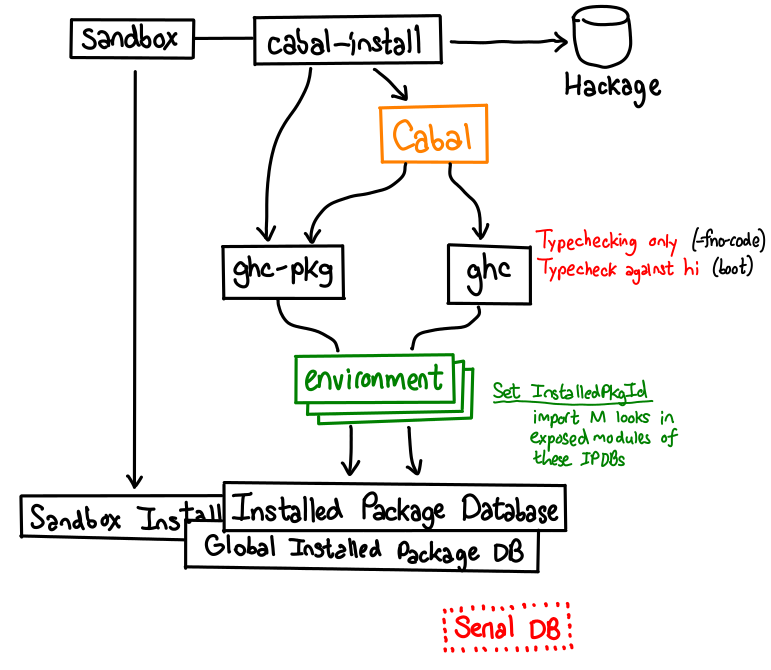
\includegraphics{arch.png}}}
\label{fig:arch}\caption{Architecture of GHC, ghc-pkg and Cabal. Green bits indicate additions from upcoming IHG work, red bits indicate additions from Backpack.  Orange indicates a Haskell library.}
\end{figure}

Here, arrows indicate dependencies from one component to another.  Color
coding is as follows: orange components are libaries, green components
are to be added with the IHG work, red components are to be added with
Backpack.  (Thus, black and orange can be considered the current)

\subsection{Installed package database}

Starting from the bottom, we have the \emph{installed package database}
(actually a collection of such databases), which stores information
about what packages have been installed are thus available to be
compiled against.  There is both a global database (for the system
administrator) and a local database (for end users), which can be
updated independently.  One way to think about the package database
is as a \emph{cache of object code}.  In principle, one could compile
any piece of code by repeatedly recompiling all of its dependencies;
the installed package database describes when this can be bypassed.

\begin{figure}[H]
    \center{\scalebox{0.8}{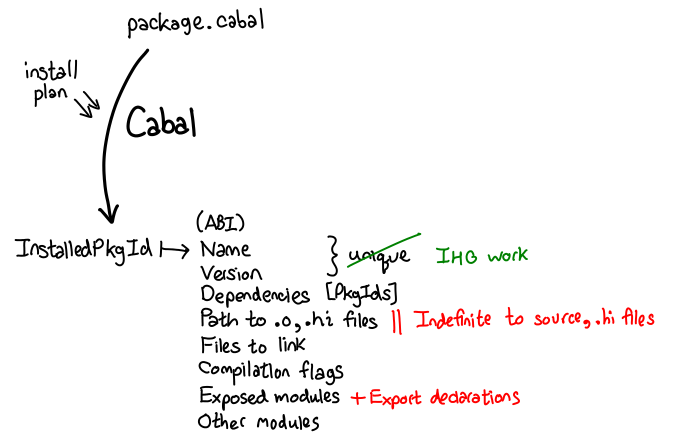
\includegraphics{pkgdb.png}}}
\label{fig:pkgdb}\caption{Anatomy of a package database.}
\end{figure}

In Figure~\ref{fig:pkgdb}, we show the structure of a package database.
The installed package are created from a Cabal file through the process
of dependency resolution and compilation.  In database terms, the primary key
of a package database is the InstalledPackageId
(Figure~\ref{fig:current-pkgid}).  This ID uniquely identifies an
instance of an installed package.  The PackageId omits the ABI hash and
is used to qualify linker exported symbols: the current value of this
parameter is communicated to GHC using the \verb|-package-id| flag.

In principle, packages with different PackageIds should be linkable
together in the same compiled program, whereas packages with the same
PackageId are not (even if they have different InstalledPackageIds).  In
practice, GHC is currently only able to select one version of a package,
as it clears out all old versions of the package in
\ghcfile{compiler/main/Package.lhs}:applyPackageFlag.

\begin{figure}
    \center{\begin{tabular}{r l}
        PackageId & package name, package version \\
        InstalledPackageId & PackageId, ABI hash \\
    \end{tabular}}
\label{fig:current-pkgid}\caption{Current structure of package identifiers.}
\end{figure}

The database entry itself contains the information from the installed package ID,
as well as information such as what dependencies it was linked against, where
its compiled code and interface files live, its compilation flags, what modules
it exposes, etc.  Much of this information is only relevant to Cabal; GHC
uses a subset of the information in the package database.

\subsection{GHC}

The two programs which access the package database directly are GHC
proper (for compilation) and ghc-pkg (which is a general purpose
command line tool for manipulating the database.)  GHC relies on
the package database in the following ways:

\begin{itemize}
    \item It imports the local and global package databases into
        its runtime database, and applies modifications to the exposed
        and trusted status of the entries via the flags \verb|-package|
        and others (\ghcfile{compiler/main/Packages.lhs}).  The internal
        package state can be seen at \verb|-v4| or higher.
    \item It uses this package database to find the location of module
        interfaces when it attempts to load the module info of an external
        module (\ghcfile{compiler/iface/LoadIface.hs}).
\end{itemize}

GHC itself performs a type checking phase, which generates an interface
file representing the module (so that later invocations of GHC can load the type
of a module), and then after compilation projects object files and linked archives
for programs to use.

\paragraph{Original names} Original names are an important design pattern
in GHC\@.
Sometimes, a name can be exposed in an hi file even if its module
wasn't exposed. Here is an example (compiled in package R):

\begin{verbatim}
module X where
    import Internal (f)
    g = f

module Internal where
    import Internal.Total (f)
\end{verbatim}

Then in X.hi:

\begin{verbatim}
g = <R.id, Internal.Total, f> (this is the original name)
\end{verbatim}

(The reason we refer to the package as R.id is because it's the
full package ID, and not just R).

\subsection{hs-boot}

\verb|hs-boot| is a special mechanism used to support recursive linking
of modules within a package, today.  Suppose I have a recursive module
dependency between modules and A and B. I break one of\ldots

(ToDo: describe how hs-boot mechanism works)

\subsection{Cabal}

Cabal is the build system for GHC, we can think of it as parsing a Cabal
file describing a package, and then making (possibly multiple)
invocations to GHC to perform the appropriate compilation.  What
information does Cabal pass onto GHC\@?  One can get an idea for this by
looking at a prototypical command line that Cabal invokes GHC with:

\begin{verbatim}
ghc --make
    -package-name myapp-0.1
    -hide-all-packages
    -package-id containers-0.9-ABCD
    Module1 Module2
\end{verbatim}

There are a few things going on here.  First, Cabal has to tell GHC
what the name of the package it's compiling (otherwise, GHC can't appropriately
generate symbols that other code referring to this package might generate).
There are also a number of commands which configure its in-memory view of
the package database (GHC's view of the package database may not directly
correspond to what is on disk).  There's also an optimization here: in principle,
GHC can compile each module one-by-one, but instead we use the \verb|--make| flag
because this allows GHC to reuse some data structures, resulting in a nontrivial
speedup.

(ToDo: describe cabal-install/sandbox)

\section{Goals}

Here are some of the high-level goals which motivate our improvements to
the module system.

\begin{itemize}
    \item Solve \emph{Cabal hell}, a situation which occurs when conflicting
        version ranges on a wide range of dependencies leads to a situation
        where it is impossible to satisfy the constraints.  We're seeking
        to solve this problem in two ways: first, we want to support
        multiple instances of containers-2.9 in the database which are
        compiled with different dependencies (and even link them
        together), and second, we want to abolish (often inaccurate)
        version ranges and move to a regime where packages depend on
        signatures.  Version ranges may still be used to indicate important
        semantic changes (e.g., bugs or bad behavior on the part of package
        authors), but they should no longer drive dependency resolution
        and often only be recorded after the fact.

    \item Support \emph{hermetic builds with sharing}.  A hermetic build
        system is one which simulates rebuilding every package whenever
        it is built; on the other hand, actually rebuilding every time
        is extremely inefficient (but what happens in practice with
        Cabal sandboxes).  We seek to solve this problem with the IHG work,
        by allowing multiple instances of a package in the database, where
        the only difference is compilation parameters.  We don't care
        about being able to link these together in a single program.

    \item Support \emph{module-level pluggability} as an alternative to
        existing (poor) usage of type classes.  The canonical example are
        strings, where a library might want to either use the convenient
        but inefficient native strings, or the efficient packed Text data
        type, but would really like to avoid having to say \verb|StringLike s => ...|
        in all of their type signatures.  While we do not plan on supporting
        separate compilation, Cabal should understand how to automatically
        recompile these ``indefinite'' packages when they are instantiated
        with a new plugin.

    \item Support \emph{separate modular development}, where a library and
        an application using the library can be developed and type-checked
        separately, intermediated by an interface.  The canonical example
        here is the \verb|ghc-api|, which is a large, complex API that
        the library writers (GHC developers) frequently change---the ability
        for downstream projects to say, ``Here is the API I'm relying on''
        without requiring these projects to actually be built would greatly
        assist in keeping the API stable. This is applicable in
        the pluggability example as well, where we want to ensure that all
        of the $M \times N$ configurations of libraries versus applications
        type check, by only running the typechecker $M + N$ times.  A closely
        related concern is related toolchain support for extracting a signature
        from an existing implementation, as current Haskell culture is averse
        to explicitly writing separate signature files.

    \item Subsume existing support for \emph{mutually recursive modules},
        without the double vision problem.
\end{itemize}

A \emph{non-goal} is to allow users to upgrade upstream libraries
without recompiling downstream. This is an ABI concern and we're not
going to worry about it.

\section{Module identities}

We are going to implement module identities slightly differently from
the way it was described from the Backpack paper. Motivated by
implementation considerations, we coarsen the
granularity of dependency tracking, so that it's not necessary to
calculate the transitive dependencies of every module: we only do it per
package.  In this next section, we recapitulate Section 3.1 of the
original Backpack paper, but with our new granularity.  Comparisons to
original Backpack will be recorded in footnotes.  Then we more generally
discuss the differing points of the design space these two occupy, and
how this affects what programs typecheck and how things are actually
implemented.

\subsection{The new scheme}

\begin{wrapfigure}{R}{0.5\textwidth}
\begin{myfig}
\[
\begin{array}{@{}lr@{\;}c@{\;}l@{}}
    \text{Package Names (\texttt{PkgName})} & P &\in& \mathit{PkgNames} \\
    \text{Module Path Names (\texttt{ModName})} & p &\in& \mathit{ModPaths} \\
    \text{Module Identity Vars} & \alpha,\beta &\in& \mathit{IdentVars} \\
    \text{Package Key (\texttt{PackageId})} & \K &::=& P(\vec{p\mapsto\nu}) \\
    \text{Module Identities (\texttt{Module})} & \nu &::=&
      \alpha ~|~
      \mu\alpha.\K\colon\! p \\
    \text{Module Identity Substs} & \phi,\theta &::=&
      \{\vec{\alpha \coloneqq \nu}\} \\
\end{array}
\]
\caption{Module Identities}
\label{fig:mod-idents}
\end{myfig}
\end{wrapfigure}

Physical module
identities $\nu$, referred to in GHC as \emph{original names}, are either (1) \emph{variables} $\alpha$, which are
used to represent holes; (2) a concrete module $p$ defined in package
$P$, with holes instantiated with other module identities (might be
empty)\footnote{In Paper Backpack, we would refer to just $P$:$p$ as the identity
constructor.  However, we've written the subterms specifically next to $P$ to highlight the semantic difference of these terms.}; or (3) \emph{recursive} module identities, defined via
$\mu$-constructors.\footnote{Actually, all concrete modules implicitly
    define a $\mu$-constructor, and we plan on using de Bruijn indices
    instead of variables in this case, a locally nameless
representation.}

As in traditional Haskell, every package contains a number of module
files at some module path $p$; within a package these paths are
guaranteed to be unique.\footnote{In Paper Backpack, the module expressions themselves are used to refer to globally unique identifiers for each literal.  This makes the metatheory simpler, but for implementation purposes it is convenient to conflate the \emph{original} module path that a module is defined at with its physical identity.}  When we write inline module definitions, we assume
that they are immediately assigned to a module path $p$ which is incorporated
into their identity.  A module identity $\nu$ simply augments this
with subterms $\vec{p\mapsto\nu}$ representing how \emph{all} holes in the package $P$
were instantiated.\footnote{In Paper Backpack, we do not distinguish between holes/non-holes, and we consider all imports of the \emph{module}, not the package.}  This naming is stable because the current Backpack surface syntax does not allow a logical path in a package
to be undefined.  A package key is $P(\vec{p\mapsto\nu})$; it is the entity
that today is internally referred to in GHC as \texttt{PackageId}.

Here is the very first example from
Section 2 of the original Backpack paper, \pname{ab-1}:

\begin{example}
\Pdef{ab-1}{
    \Pmod{A}{x = True}
    \Pmod{B}{\Mimp{A}; y = not x}
    % \Pmodd{C}{\mname{A}}
}
\end{example}

The identities of \m{A} and \m{B} are
\pname{ab-1}:\mname{A} and \pname{ab-1}:\mname{B}, respectively.\footnote{In Paper Backpack, the identity for \mname{B} records its import of \mname{A}, but since it is definite, this is strictly redundant.} In a package with holes, each
hole gets a fresh variable (within the package definition) as its
identity, and all of the holes associated with package $P$ are recorded. Consider \pname{abcd-holes-1}:

\begin{example}
\Pdef{abcd-holes-1}{
    \Psig{A}{x :: Bool} % chktex 26
    \Psig{B}{y :: Bool} % chktex 26
    \Pmod{C}{x = False}
    \Pmodbig{D}{
        \Mimpq{A}\\
        \Mimpq{C}\\
        % \Mexp{\m{A}.x, z}\\
        z = \m{A}.x \&\& \m{C}.x
    }
}
\end{example}

The identities of the four modules
are, in order, $\alpha_a$, $\alpha_b$, $\pname{abcd-holes-1}(\alpha_a,\alpha_b)$:\mname{C}, and
$\pname{abcd-holes-1}(\alpha_a,\alpha_b)$:\mname{D}.\footnote{In Paper Backpack, the granularity is at the module level, so the subterms of \mname{C} and \mname{D} can differ.}

Consider now the module identities in the \m{Graph} instantiations in
\pname{multinst}, shown in Figure 2 of the original Backpack paper (we have
omitted it for brevity).
In the definition of \pname{structures}, assume that the variables for
\m{Prelude} and \m{Array} are $\alpha_P$ and $\alpha_A$ respectively.
The identity of \m{Graph} is $\pname{structures}(\alpha_P, \alpha_A)$:\m{Graph}. Similarly, the identities of the two array implementations
are $\nu_{AA} = \pname{arrays-a}(\alpha_P)$:\m{Array} and
$\nu_{AB} = \pname{arrays-b}(\alpha_P)$:\m{Array}.\footnote{Notice that the subterms coincide with Paper Backpack!  A sign that module level granularity is not necessary for many use-cases.}

The package \pname{graph-a} is more interesting because it
\emph{links} the packages \pname{arrays-a} and \pname{structures}
together, with the implementation of \m{Array} from \pname{arrays-a}
\emph{instantiating} the hole \m{Array} from \pname{structures}.  This
linking is reflected in the identity of the \m{Graph} module in
\pname{graph-a}: whereas in \pname{structures} it was $\nu_G =
\pname{structures}(\alpha_P, \alpha_A)$:\m{Graph}, in \pname{graph-a} it is
$\nu_{GA} = \nu_G[\nu_{AA}/\alpha_A] = \pname{structures}(\alpha_P, \nu_{AA})$:\m{Graph}.  Similarly, the identity of \m{Graph} in
\pname{graph-b} is $\nu_{GB} = \nu_G[\nu_{AB}/\alpha_A] =
\pname{structures}(\alpha_P, \nu_{AB})$:\m{Graph}.  Thus, linking consists
of substituting the variable identity of a hole by the concrete
identity of the module filling that hole.

Lastly, \pname{multinst} makes use of both of these \m{Graph}
modules, under the aliases \m{GA} and \m{GB}, respectively.
Consequently, in the \m{Client} module, \code{\m{GA}.G} and
\code{\m{GB}.G} will be correctly viewed as distinct types since they
originate in modules with distinct identities.

As \pname{multinst} illustrates, module identities effectively encode
dependency graphs at the package level.\footnote{In Paper Backpack, module identities
encode dependency graphs at the module level.  In both cases, however, what is being
depended on is always a module.}  Like in Paper Backpack, we have an \emph{applicative}
semantics of instantiation, and the applicativity example in Figure 3 of the
Backpack paper still type checks.  However, because we are operating at a coarser
granularity, modules may have spurious dependencies on holes that they don't
actually depend on, which means less type equalities may hold.

Shaping proceeds in the same way as in Paper Backpack, except that the
shaping judgment must also accept the package key
$P(\vec{p\mapsto\alpha})$ so we can create identifiers with
\textsf{mkident}.  This implies we must know ahead of time what the holes
of a package are.

\subsection{Commentary}

\begin{wrapfigure}{r}{0.4\textwidth}
\begin{verbatim}
package p where
    A :: ...
    -- B does not import A
    B = [ data T = T; f T = T ]
    C = [ import A; ... ]
package q where
    A1 = [ ... ]
    A2 = [ ... ]
    include p (A as A1, B as B1)
    include p (A as A2, B as B2)
    Main = [
        import qualified B1
        import qualified B2
        y = B1.f B2.T
    ]
\end{verbatim}
\caption{The difference between package and module granularity}\label{fig:granularity}
\end{wrapfigure}

\paragraph{The sliding scale of granularity}  The scheme we have described
here is coarser-grained than Backpack's, and thus does not accept as many
programs.  Figure~\ref{fig:granularity} is a minimal example which doesn't type
check in our new scheme.
In Paper Backpack, the physical module identities of \m{B1} and \m{B2} are
both $\K_B$, and so \m{Main} typechecks.  However, in GHC Backpack,
we assign module identities $\pname{p(q:A1)}$:$\m{B}$ and $\pname{p(q:A2)}$:$\m{B}$,
which are not equal.

Does this mean that Paper Backpack's form of granularity is \emph{better?}
Not necessarily!  First, we can always split packages into further subpackages
which better reflect the internal hole dependencies, so it is always possible
to rewrite a program to make it typecheck---just with more packages.  Second,
Paper Backpack's granularity is only one on a sliding scale; it is by no means
the most extreme!  You could imagine a version of Backpack where we desugared
each \emph{expression} into a separate module.\footnote{Indeed, there are some
languages which take this stance. (See Bob Harper's work.)}  Then, even if \m{B} imported
\m{A}, as long as it didn't use any types from \m{A} in the definition of
\verb|T|, we would still consider the types equal.  Finally, to understand
what the physical module identity of a module is, in Paper Backpack I must
understand the internal dependency structure of the modules in a package. This
is a lot of work for the developer to think about; a more granular model
is also easier to reason about.

Nevertheless, finer granularity can be desirable from an end-user perspective.
Usually, these circumstances arise when library-writers are forced to split their
components into many separate packages, when they would much rather have written
a single package.  For example, if I define a data type in my library, and would
like to define a \verb|Lens| instance for it, I would create a new package just
for the instance, in order to avoid saddling users who aren't interested in lenses
with an extra dependency.  Another example is test suites, which have dependencies
on various test frameworks that a user won't care about if they are not planning
on testing the code. (Cabal has a special case for this, allowing the user
to write effectively multiple packages in a single Cabal file.)

\paragraph{Cabal dependency resolution}  Currently, when we compile a Cabal
package, Cabal goes ahead and resolves \verb|build-depends| entries with actual
implementations, which we compile against.  A planned addition to the package key,
independent of Backpack, is to record the transitive dependency tree selected
during this dependency resolution process, so that we can install \pname{libfoo-1.0}
twice compiled against different versions of its dependencies.
What is the relationship to this transitive dependency tree of \emph{packages},
with the subterms of our package identities which are \emph{modules}?  Does one
subsume the other?  In fact, these are separate mechanisms---two levels of indirections,
so to speak.

To illustrate, suppose I write a Cabal file with \verb|build-depends: foobar|.  A reasonable assumption is that this translates into a
Backpack package which has \verb|include foobar|.  However, this is not
actually a Paper Backpack package: Cabal's dependency solver has to
rewrite all of these package references into versioned references
\verb|include foobar-0.1|.  For example, this is a pre-package:

\begin{verbatim}
package foo where
    include bar
\end{verbatim}

and this is a Paper Backpack package:

\begin{verbatim}
package foo-0.3[bar-0.1[baz-0.2]] where
    include bar-0.1[baz-0.2]
\end{verbatim}

This tree is very similar to the one tracking dependencies for holes,
but we must record this tree \emph{even} when our package has no holes.
As a final example, the full module
identity of \m{B1} in Figure~\ref{fig:granularity} may actually be $\pname{p-0.9(q-1.0[p-0.9]:A1)}$:\m{B}.

\subsection{Implementation}

In GHC's current packaging system, a single package compiles into a
single entry in the installed package database, indexed by the package
key.  This property is preserved by package-level granularity, as we
assign the same package key to all modules.  Package keys provide an
easy mechanism for sharing to occur: when an indefinite package is fully
instantiated, we can check if we already have its package key installed
in the installed package database.  (At the end of this section, we'll
briefly discuss some of the problems actually implementing Paper Backpack.)
It is also important to note that we are \emph{willing to duplicate code};
processes like this already happen in other parts of the compiler
(such as inlining.)

However, there is one major challenge for this scheme, related to
\emph{dynamically linked libraries}.  Consider this example:

\begin{verbatim}
package p where
    A :: [ ... ]
    B = [ ... ]
package q where
    A = [ ... ]
    include p
    C = [ import A; import B; ... ]
\end{verbatim}

When we compile package \pname{q}, we end up compiling package keys
\pname{q} and $\pname{p(q:A)}$, which turn into their respective libraries
in the installed package database.  When we need to statically link against
these libraries, it doesn't matter that \pname{q} refers to code in $\pname{p(q:A)}$,
and vice versa: the linker is building an executable and can resolve all
of the symbols in one go.  However, when the libraries in question are
dynamic libraries \verb|libHSq.so| and \verb|libHSp(q:A).so|, this is now
a \emph{circular dependency} between the two libraries, and most dynamic
linkers will not be able to load either of these libraries.

Our plan is to break the circularity by inlining the entire module \m{A}
into $\pname{p(q:A)}$ when it is necessary (perhaps in other situations,
\m{A} will be in another package and no inlining is necessary).  The code
in both situations should be exactly the same, so it should be completely
permissible to consider them type-equal.

\paragraph{Relaxing package selection restrictions}  As mentioned
previously, GHC is unable to select multiple packages with the same
package name (but different package keys).  This restriction needs to be
lifted.  We should add a new flag \verb|-package-key|.  GHC also knows
about version numbers and will mask out old versions of a library when
you make another version visible; this behavior needs to be modified.

\paragraph{Linker symbols} As we increase the amount of information in
PackageId, it's important to be careful about the length of these IDs,
as they are used for exported linker symbols (e.g.
\verb|base_TextziReadziLex_zdwvalDig_info|).  Very long symbol names
hurt compile and link time, object file sizes, GHCi startup time,
dynamic linking, and make gdb hard to use.  As such, the current plan is
to do away with full package names and versions, and instead use just a
base-62 encoded hash, perhaps with the first four characters of the package
name for user-friendliness.

\paragraph{Wired-in names} One annoying thing to remember is that GHC
has wired-in names, which refer to packages without any version.  These
are specially treated during compilation so that they are built using
a package key that has no version or dependency information.  One approach
is to continue treating these libraries specially; alternately we can
maintain a fixed table from these wired names to
package IDs.

\section{Shapeless Backpack}\label{sec:simplifying-backpack}

Backpack as currently defined always requires a \emph{shaping} pass,
which calculates the shapes of all modules defined in a package.
The shaping pass is critical to the solution of the double-vision problem
in recursive module linking, but it also presents a number of unpalatable
implementation problems:

\begin{itemize}

    \item \emph{Shaping is a lot of work.} A module shape specifies the
        providence of all data types and identifiers defined by a
        module. To calculate this, we must preprocess and parse all
        modules, even before we do the type-checking pass.  (Fortunately,
        shaping doesn't require a full parse of a module, only enough
        to get identifiers.  However, it does have to understand import
        statements at the same level of detail as GHC's renamer.)

    \item \emph{Shaping must be done upfront.} In the current Backpack
        design, all shapes must be computed before any typechecking can
        occur.  While performing the shaping pass upfront is necessary
        in order to solve the double vision problem (where a module
        identity may be influenced by later definitions), it means
        that GHC must first do a shaping pass, and then revisit every module and
        compile them proper.  Nor is it (easily) possible to skip the
        shaping pass when it is unnecessary, as one might expect to be
        the case in the absence of mutual recursion.  Shaping is not
        a ``pay as you go'' language feature.

    \item \emph{GHC can't compile all programs shaping accepts.}  Shaping
        accepts programs that GHC, with its current hs-boot mechanism, cannot
        compile.  In particular, GHC requires that any data type or function
        in a signature actually be \emph{defined} in the module corresponding
        to that file (i.e., an original name can be assigned to these entities
        immediately.)  Shaping permits unrestricted exports to implement
        modules; this shows up in the formalism as $\beta$ module variables.

    \item \emph{Shaping encourages inefficient program organization.}
        Shaping is designed to enable mutually recursive modules, but as
        currently implemented, mutual recursion is less efficient than
        code without recursive dependencies. Programmers should avoid
        this code organization, except when it is absolutely necessary.

    \item \emph{GHC is architecturally ill-suited for directly
        implementing shaping.}  Shaping implies that GHC's internal
        concept of an ``original name'' be extended to accommodate
        module variables.  This is an extremely invasive change to all
        aspects of GHC, since the original names assumption is baked
        quite deeply into the compiler.  Plausible implementations of
        shaping requires all these variables to be skolemized outside
        of GHC\@.

\end{itemize}

To be clear, the shaping pass is fundamentally necessary for some
Backpack packages.  Here is the example which convinced Simon:

\begin{verbatim}
package p where
    A :: [data T; f :: T -> T]
    B = [export T(MkT), h; import A(f); data T = MkT; h x = f MkT]
    A = [export T(MkT), f, h; import B; f MkT = MkT]
\end{verbatim}

The key to this example is that B \emph{may or may not typecheck} depending
on the definition of A. Because A reexports B's definition T, B will
typecheck; but if A defined T on its own, B would not typecheck.  Thus,
we \emph{cannot} typecheck B until we have done some analysis of A (the
shaping analysis!)

Thus, it is beneficial (from an optimization point of view) to
consider a subset of Backpack for which shaping is not necessary.
Here is a programming discipline which does just that, which we will call the \textbf{linking restriction}: \emph{Module implementations must be declared before
signatures.}  Formally, this restriction modifies the rule for merging
polarized module shapes ($\widetilde{\tau}_1^{m_1} \oplus \widetilde{\tau}_2^{m_2}$) so that
$\widetilde{\tau}_1^- \oplus \widetilde{\tau}_2^+$ is always undefined.\footnote{This seemed to be the crispest way of defining the restriction, although this means an error happens a bit later than I'd like it to: I'd prefer if we errored while merging logical contexts, but we don't know what is a hole at that point.}

Here is an example of the linking restriction. Consider these two packages:

\begin{verbatim}
package random where
    System.Random = [ ... ].hs

package monte-carlo where
    System.Random :: ...
    System.MonteCarlo = [ ... ].hs
\end{verbatim}

Here, random is a definite package which may have been compiled ahead
of time; monte-carlo is an indefinite package with a dependency
on any package which provides \verb|System.Random|.

Now, to link these two applications together, only one ordering
is permissible:

\begin{verbatim}
package myapp where
    include random
    include monte-carlo
\end{verbatim}

If myapp wants to provide its own random implementation, it can do so:

\begin{verbatim}
package myapp2 where
    System.Random = [ ... ].hs
    include monte-carlo
\end{verbatim}

In both cases, all of \verb|monte-carlo|'s holes have been filled in by the time
it is included.  The alternate ordering is not allowed.

Why does this discipline prevent mutually recursive modules?  Intuitively,
a hole is the mechanism by which we can refer to an implementation
before it is defined; otherwise, we can only refer to definitions which
preceed our definition. If there are never any holes \emph{which get filled},
implementation links can only go backwards, ruling out circularity.

It's easy to see how mutual recursion can occur if we break this discipline:

\begin{verbatim}
package myapp2 where
    include monte-carlo
    System.Random = [ import System.MonteCarlo ].hs
\end{verbatim}

\subsection{Typechecking of definite modules without shaping}

If we are not carrying out a shaping pass, we need to be able to calculate
$\widetilde{\Xi}_{\mathsf{pkg}}$ on the fly.  In the case that we are
compiling a package---there will be no holes in the final package---we
can show that shaping is unnecessary quite easily, since with the
linking restriction, everything is definite from the get-go.

Observe the following invariant: at any given step of the module
bindings, the physical context $\widetilde{\Phi}$ contains no
holes.  We can thus conclude that there are no module variables in any
type shapes.  As the only time a previously calculated package shape can
change is due to unification, the incrementally computed shape is in
fact the true one.

As far as the implementation is concerned, we never have to worry
about handling module variables; we only need to do extra typechecks
against (renamed) interface files.

\subsection{Compilation of definite modules}\label{sec:compiling-definite}

Of course, we still have to compile the code, and this includes any
subpackages which we have mixed in the dependencies to make them fully
definite.  Let's take the following set of packages as an example:

\begin{verbatim}
package pkg-a where
    A = [ a = 0; b = 0 ] -- b is not visible
    B = ... -- this code is ignored
package pgk-b where -- indefinite package
    A :: [ a :: Bool ]
    B = [ import A; b = 1 ]
package pkg-c where
    include pkg-a (A)
    include pkg-b
    C = [ import B; ... ]
\end{verbatim}

Note: in the following example, we will assume that we are operating
under the packaging scheme specified in Section~\ref{sec:one-per-definite-package}
with the indefinite package refinement.

With the linking invariant, we can simply walk the Backpack package ``tree'',
compiling each of its dependencies.  Let's walk through it explicitly.\footnote{To simplify matters, we assume that there is only one instance of any
PackageId in the database, so we omit the unique-ifying hashes from the
ghc-pkg registration commands; we ignore the existence of version numbers
and Cabal's dependency solver; finally, we do the compilation in
one-shot mode, even though Cabal in practice will use the Make mode.}

First, we have to build \verb|pkg-a|.  This package has no dependencies
of any kind, so compiling is much like compiling ordinary Haskell.  If
it was already installed in the database, we wouldn't even bother compiling it.

\begin{verbatim}
ADEPS =    # empty!
ghc -c A.hs -package-name pkg-a-ADEPS
ghc -c B.hs -package-name pkg-a-ADEPS
# install and register pkg-a-ADEPS
\end{verbatim}

Next, we have to build \verb|pkg-b|.  This package has a hole \verb|A|,
intuitively, it depends on package A.   This is done in two steps:
first we check if the signature given for the hole matches up with the
actual implementation provided. Then we build the module properly.

\begin{verbatim}
BDEPS = "A -> pkg-a-ADEPS:A"
ghc -c A.hs-boot -package-name pkg-b-BDEPS -hide-all-packages \
    -package "pkg-a-ADEPS(A)"
ghc -c B.hs      -package-name pkg-b-BDEPS -hide-all-packages \
    -package "pkg-a-ADEPS(A)"
# install and register pkg-b-BDEPS
\end{verbatim}

These commands mostly resemble the traditional compilation process, but
with some minor differences.  First, the \verb|-package| includes must
also specify a thinning (and renaming) list.  This is because when
\verb|pkg-b| is compiled, it only sees module \verb|A| from it, not
module \verb|B| (as it was thinned out.)  Conceptually, this package is
being compiled in the context of some module environment \verb|BDEPS| (a
logical context, in Backpack lingo) which maps modules to original names
and is utilized by the module finder to lookup the import in
\verb|B.hs|; we load/thin/rename packages so that the package
environment accurately reflects the module environment.

Similarly, it is important that the compilation of \verb|B.hs| use \verb|A.hi-boot|
to determine what entities in the module are visible upon import; this is
automatically detected by \verb|GHC| when the compilation occurs.  Otherwise,
in module \verb|pkg-b:B|, there would be a name collision between the local
definition of \verb|b| and the identifier \verb|b| which was
accidentally pulled in when we compiled against the actual implementation of
\verb|A|.  It's actually a bit tempting to compile \verb|pkg-b:B| against the
\verb|hi-boot| generated by the signature, but this would unnecessarily
lose out on possible optimizations which are stored in the original \verb|hi|
file, but not evident from \verb|hi-boot|.

Finally, we created all of the necessary subpackages, and we can compile
our package proper.

\begin{verbatim}
CDEPS =         # empty!!
ghc -c C.hs -package-name pkg-c-CDEPS -hide-all-packages \
    -package "pkg-a-ADEPS(A)" \
    -package "pkg-b-BDEPS"
# install and register package pkg-c-CDEPS
\end{verbatim}

This command is quite similar, although it's worth mentioning that now,
the \verb|package| flags directly mirror the syntax in Backpack.
Additionally, even though \verb|pkg-c| ``depends'' on subpackages, these
do not show in its package-name identifier, e.g. CDEPS\@.  This is
because this package \emph{chose} the values of ADEPS and BDEPS
explicitly (by including the packages in this particular order), so
there are no degrees of freedom.\footnote{In the presence of a
    Cabal-style dependency solver which associates a-0.1 with a concrete
identifier a, these choices need to be recorded in the package ID.}

Overall, there are a few important things to notice about this architecture.
First, because the \verb|pkg-b-BDEPS| product is installed, if in another package
build we instantiate the indefinite module B with exactly the same \verb|pkg-a|
implementation, we can skip the compilation process and reuse the version.
This is because the calculated \verb|BDEPS| will be the same, and thus the package
IDs will be the same.

XXX ToDo: actually write down pseudocode algorithm for this

\paragraph{Sometimes you need a module environment instead}  In the compilation
description here, we've implicitly assumed that any external modules you might
depend on exist in a package somewhere.  However, a tricky situation
occurs when some of these modules come from a parent package:
\begin{verbatim}
package pkg-b where
    A :: [ a :: Bool ]
    B = [ import A; b = 1 ]
package pkg-c where
    A = [ a = 0; b = 0 ]
    include pkg-b
    C = [ import B; ... ]
\end{verbatim}

How this problem gets resolved depends on what our library granularity is (Section~\ref{sec:flatten}).

In the ``only definite packages are compiled'' world
(Section~\ref{sec:one-per-definite-package}), we need to pass a
special ``module environment'' to the compilation of libraries
in \verb|monte-carlo| to say where to find \verb|System.Random|.
The compilation of \verb|pkg-b| now looks as follows:

\begin{verbatim}
BDEPS = "A -> pkg-a-ADEPS:A"
ghc -c A.hs-boot -package-name pkg-a-ADEPS -module-env BDEPS
ghc -c B.hs      -package-name pkg-a-ADEPS -subpackage-name pkg-b-BDEPS -module-env BDEPS
\end{verbatim}

The most important thing to remember here is that in the ``only definite
packages are compiled'' world, we must create a \emph{copy} of
\verb|pkg-b| in order to instantiate its hole with \verb|pkg-a:A|
(otherwise, there is a circular dependency.)  These packages must be
distinguished from the parent package (\verb|-subpackage-name|), but
logically, they will be installed in the \verb|pkg-a| library.  The
module environment specifies where the holes can be found, without
referring to an actual package (since \verb|pkg-a| has, indeed, not been
installed yet at the time we process \verb|B.hs|).  These files are
probably looked up in the include paths.\footnote{It's worth remarking
    that a variant of this was originally proposed as the one true
    compilation strategy.  However, it was pointed out that this gave up
    applicativity in all cases.  Our current refinement of this strategy
gives up applicativity for modules which have not been placed in an
external package.}

Things are a bit different in sliced world and physical module identity
world (Section~\ref{sec:one-per-package-identity}); here, we really do
compile and install (perhaps to a local database) \verb|pkg-c:A| before
starting with the compilation of \verb|pkg-b|.  So package imports will
continue to work fine.

\subsection{Restricted recursive modules ala hs-boot}\label{sec:hs-boot-restrict}

It should be possible to support GHC-style mutual recursion using the
Backpack formalism immediately using hs-boot files.  However, to avoid
the need for a shaping pass, we must adopt an existing constraint that
already applies to hs-boot files: \emph{at the time we define a signature,
we must know what the original name for all data types is}.  In practice,
GHC enforces this by stating that: (1) an hs-boot file must be
accompanied with an implementation, and (2) the implementation must
in fact define (and not reexport) all of the declarations in the signature.

Why does this not require a shaping pass? The reason is that the
signature is not really polymorphic: we require that the $\alpha$ module
variable be resolved to a concrete module later in the same package, and
that all the $\beta$ module variables be unified with $\alpha$. Thus, we
know ahead of time the original names and don't need to deal with any
renaming.\footnote{This strategy doesn't completely resolve the problem
of cross-package mutual recursion, because we need to first compile a
bit of the first package (signatures), then the second package, and then
the rest of the first package.}

Compiling packages in this way gives the tantalizing possibility
of true separate compilation: the only thing we don't know is what the actual
package name of an indefinite package will be, and what the correct references
to have are.  This is a very minor change to the assembly, so one could conceive
of dynamically rewriting these references at the linking stage.  But
separate compilation achieved in this fashion would not be able to take
advantage of cross-module optimizations.

\section{Shaped Backpack}

Despite the simplicity of shapeless Backpack with the linking
restriction in the absence of holes, we will find that when we have
holes, it will be very difficult to do type-checking without
some form of shaping.  This section is very much a work in progress,
but the ability to typecheck against holes, even with the linking restriction,
is a very important part of modular separate development, so we will need
to support it at some ponit.

\subsection{Efficient shaping}

(These are Edward's opinion, he hasn't convinced other folks that this is
the right way to do it.)

In this section, I want to argue that, although shaping constitutes
a pre-pass which must be run before compilation in earnest, it is only
about as bad as the dependency resolution analysis that GHC already does
in \verb|ghc -M| or \verb|ghc --make|.

In Paper Backpack, what information does shaping compute? It looks at
exports, imports, data declarations and value declarations (but not the
actual expressions associated with these values.)  As a matter of fact,
GHC already must look at the imports associated with a package in order
to determine the dependency graph, so that it can have some order to compile
modules in.  There is a specialized parser which just parses these statements,
and then ignores the rest of the file.

A bit of background: the \emph{renamer} is responsible for resolving
imports and figuring out where all of these entities actually come from.
SPJ would really like to avoid having to run the renamer in order to perform
a shaping pass.

\paragraph{Is it necessary to run the Renamer to do shaping?}
Edward and Scott believe the answer is no, well, partially.
Shaping needs to know the original names of all entities exposed by a
module/signature. Then it needs to know (a) which entities a module/signature
defines/declares locally and (b) which entities that module/signature exports.
The former, (a), can be determined by a straightforward inspection of a parse
tree of the source file.\footnote{Note that no expression or type parsing
is necessary. We only need names of local values, data types, and data
constructors.} The latter, (b), is a bit trickier. Right now it's the Renamer
that interprets imports and exports into original names, so we would still
rely on that implementation. However, the Renamer does other, harder things
that we don't need, so ideally we could factor out the import/export
resolution from the Renamer for use in shaping.

Unfortunately the Renamer's import resolution analyzes \verb|.hi| files, but for
local modules, which haven't yet been typechecked, we don't have those.
Instead, we could use a new file format, \verb|.hsi| files, to store the shape of
a locally defined module. (Defined packages are bundled with their shapes,
so included modules have \verb|.hsi| files as well.) (What about the logical
vs.~physical distinction in file names?) If we refactor the import/export
resolution code, could we rewrite it to generically operate on both
\verb|.hi| files and \verb|.hsi| files?

Alternatively, rather than storing shapes on a per-source basis, we could
store (in memory) the entire package shape. Similarly, included packages
could have a single shape file for the entire package. Although this approach
would make shaping non-incremental, since an entire package's shape would
be recomputed any time a constituent module's shape changes, we do not expect
shaping to be all that expensive.

\subsection{Typechecking of indefinite modules}\label{sec:typechecking-indefinite}

Recall in our argument in the definite case, where we showed there are
no holes in the physical context.  With indefinite modules, this is no
longer true. While (with the linking restriction) these holes will never
be linked against a physical implementation, they may be linked against
other signatures.  (Note: while disallowing signature linking would
solve our problem, it would disallow a wide array of useful instances of
signature reuse, for example, a package mylib that implements both
mylib-1x-sig and mylib-2x-sig.)

With holes, we must handle module variables, and we sometimes must unify them:

\begin{verbatim}
package p where
    A :: [ data A ]
package q where
    A :: [ data A ]
package r where
    include p
    include q
\end{verbatim}

In this package, it is not possible to a priori assign original names to
module A in p and q, because in package r, they should have the same
original name.  When signature linking occurs, unification may occur,
which means we have to rename all relevant original names. (A similar
situation occurs when a module is typechecked against a signature.)

An invariant which would be nice to have is this: when typechecking a
signature or including a package, we may apply renaming to the entities
being brought into context.  But once we've picked an original name for
our entities, no further renaming should be necessary. (Formally, in the
unification for semantic object shapes, apply the unifier to the second
shape, but not the first one.)

However, there are plenty of counterexamples here:

\begin{verbatim}
package p where
    A :: [ data A ]
    B :: [ data A ]
    M = ...
    A = B
\end{verbatim}

In this package, does module M know that A.A and B.A are type equal?  In
fact, the shaping pass will have assigned equal module identities to A
and B, so M \emph{equates these types}, despite the aliasing occurring
after the fact.

We can make this example more sophisticated, by having a later
subpackage which causes the aliasing; now, the decision is not even a
local one (on the other hand, the equality should be evident by inspection
of the package interface associated with q):

\begin{verbatim}
package p where
    A :: [ data A ]
    B :: [ data A ]
package q where
    A :: [ data A ]
    B = A
package r where
    include p
    include q
\end{verbatim}

Another possibility is that it might be acceptable to do a mini-shaping
pass, without parsing modules or signatures, \emph{simply} looking at
names and aliases.  But logical names are not the only mechanism by
which unification may occur:

\begin{verbatim}
package p where
    C :: [ data A ]
    A = [ data A = A ]
    B :: [ import A(A) ]
    C = B
\end{verbatim}

It is easy to conclude that the original names of C and B are the same.  But
more importantly, C.A must be given the original name of p:A.A.  This can only
be discovered by looking at the signature definition for B. In any case, it
is worth noting that this situation parallels the situation with hs-boot
files (although there is no mutual recursion here).

The conclusion is that you will probably, in fact, have to do real
shaping in order to typecheck all of these examples.

\paragraph{Hey, these signature imports are kind of tricky\ldots}

When signatures and modules are interleaved, the interaction can be
complex.  Here is an example:

\begin{verbatim}
package p where
    C :: [ data A ]
    M = [ import C; ... ]
    A = [ import M; data A = A ]
    C :: [ import A(A) ]
\end{verbatim}

Here, the second signature for C refers to a module implementation A
(this is permissible: it simply means that the original name for p:C.A
is p:A.A).  But wait! A relies on M, and M relies on C. Circularity?
Fortunately not: a client of package p will find it impossible to have
the hole C implemented in advance, since they will need to get their hands on module
A\ldots but it will not be defined prior to package p.

In any case, however, it would be good to emit a warning if a package
cannot be compiled without mutual recursion.

\subsection{Incremental typechecking}
We want to typecheck modules incrementally, i.e., when something changes in
a package, we only want to re-typecheck the modules that care about that
change. GHC already does this today.%
\footnote{\url{https://ghc.haskell.org/trac/ghc/wiki/Commentary/Compiler/RecompilationAvoidance}}
Is the same mechanism sufficient for Backpack? Edward and Scott think that it
is, mostly. Our conjecture is that a module should be re-typechecked if the
existing mechanism says it should \emph{or} if the logical shape
context (which maps logical names to physical names) has changed. The latter
condition is due to aliases that affect typechecking of modules.

Let's look again at an example from before:
\begin{verbatim}
package p where
    A :: [ data A ]
    B :: [ data A ]
    M = [ import A; import B; ... ]
\end{verbatim}
Let's say that \verb|M| is typechecked successfully. Now we add an alias binding
at the end of the package, \verb|A = B|. Does \verb|M| need to be
re-typechecked? Yes! (Well, it seems so, but let's just assert ``yes'' for now.
Certainly in the reverse case---if we remove the alias and then ask---this
is true, since \verb|M| might have depended on the two \verb|A| types
being the same.)
The logical shape context changed to say that \verb|A| and
\verb|B| now map to the same physical module identity. But does the existing
recompilation avoidance mechanism say that \verb|M| should be re-typechecked?
It's unclear. The \verb|.hi| file for \verb|M| records that it imported \verb|A| and
\verb|B| with particular ABIs, but does it also know about the physical module
identities (or rather, original module names) of these modules?

Scott thinks this highlights the need for us to get our story straight about
the connection between logical names, physical module identities, and file
names!


\subsection{Installing indefinite packages}\label{sec:installing-indefinite}

If an indefinite package contains no code at all, we only need
to install the interface file for the signatures.  However, if
they include code, we must provide all of the
ingredients necessary to compile them when the holes are linked against
actual implementations.  (Figure~\ref{fig:pkgdb})

\paragraph{Source tarball or preprocessed source?}  What is the representation of the source that is saved is.  There
are a number of possible choices:

\begin{itemize}
    \item The original tarballs downloaded from Hackage,
    \item Preprocessed source files,
    \item Some sort of internal, type-checked representation of Haskell code (maybe the output of the desugarer).
\end{itemize}

Storing the tarballs is the simplest and most straightforward mechanism,
but we will have to be very certain that we can recompile the module
later in precisely the same we compiled it originally, to ensure the hi
files match up (fortunately, it should be simple to perform an optional
sanity check before proceeding.) The appeal of saving preprocessed
source, or even the IRs, is that this is conceptually this is exactly
what an indefinite package is: we have paused the compilation process
partway, intending to finish it later.  However, our compilation strategy
for definite packages requires us to run this step using a \emph{different}
choice of original names, so it's unclear how much work could actually be reused.

\section{Surface syntax}

In the Backpack paper, a brand new module language is presented, with
syntax for inline modules and signatures.  This syntax is probably worth implementing,
because it makes it easy to specify compatibility packages, whose module
definitions in general may be very short:

\begin{verbatim}
package ishake-0.12-shake-0.13 where
    include shake-0.13
    Development.Shake.Sys = Development.Shake.Cmd
    Development.Shake = [ (**>) = (&>) ; (*>>) = (|*>)]
    Development.Shake.Rule = [ defaultPriority = rule . priority 0.5 ]
    include ishake-0.12
\end{verbatim}

However, there are a few things that are less than ideal about the
surface syntax proposed by Paper Backpack:

\begin{itemize}
    \item It's completely different from the current method users
        specify packages. There's nothing wrong with this per se
        (one simply needs to support both formats) but the smaller
        the delta, the easier the new packaging format is to explain
        and implement.

    \item Sometimes order matters (relative ordering of signatures and
        module implementations), and other times it does not (aliases).
        This can be confusing for users.

    \item Users have to order module definitions topologically,
        whereas in current Cabal modules can be listed in any order, and
        GHC figures out an appropriate order to compile them.
\end{itemize}

Here is an alternative proposal, closely based on Cabal syntax.  Given
the following Backpack definition:

\begin{verbatim}
package libfoo(A, B, C, Foo) where
    include base
    -- renaming and thinning
    include libfoo (Foo, Bar as Baz)
    -- holes
    A :: [ a :: Bool ].hsig
    A2 :: [ b :: Bool ].hsig
    -- normal module
    B = [
        import {-# SOURCE #-} A
        import Foo
        import Baz
        ...
    ].hs
    -- recursively linked pair of modules, one is private
    C :: [ data C ].hsig
    D = [ import {-# SOURCE #-} C; data D = D C ].hs
    C = [ import D; data C = C D ].hs
    -- alias
    A = A2
\end{verbatim}

We can write the following Cabal-like syntax instead (where
all of the signatures and modules are placed in appropriately
named files):

\begin{verbatim}
package: libfoo
...
build-depends: base, libfoo (Foo, Bar as Baz)
holes: A A2 -- deferred for now
exposed-modules: Foo B C
aliases: A = A2
other-modules: D
\end{verbatim}

Notably, all of these lists are \emph{insensitive} to ordering!
The key idea is use of the \verb|{-# SOURCE #-}| pragma, which
is enough to solve the important ordering constraint between
signatures and modules.

Here is how the elaboration works.  For simplicity, in this algorithm
description, we assume all packages being compiled have no holes
(including \verb|build-depends| packages). Later, we'll discuss how to
extend the algorithm to handle holes in both subpackages and the main
package itself.

\begin{enumerate}

    \item At the top-level with \verb|package| $p$ and
        \verb|exposed-modules| $ms$, record \verb|package p (ms) where|

    \item For each package $p$ with thinning/renaming $ms$ in
        \verb|build-depends|, record a \verb|include p (ms)| in the
        Backpack package.  The ordering of these includes does not
        matter, since none of these packages have holes.

    \item Take all modules $m$ in \verb|other-modules| and
        \verb|exposed-modules| which were not exported by build
        dependencies, and create a directed graph where hs and hs-boot
        files are nodes and imports are edges (the target of an edge is
        an hs file if it is a normal import, and an hs-boot file if it
        is a SOURCE import).  Topologically sort this graph, erroring if
        this graph contains cycles (even with recursive modules, the
        cycle should have been broken by an hs-boot file).  For each
        node, in this order, record \verb|M = [ ... ]| or \verb|M :: [ ... ]|
        depending on whether or not it is an hs or hs-boot.  If possible,
        sort signatures before implementations when there is no constraint
        otherwise.

\end{enumerate}

Here is a simple example which shows how SOURCE can be used to disambiguate
between two important cases. Suppose we have these modules:

\begin{verbatim}
-- A1.hs
import {-# SOURCE #-} B

-- A2.hs
import B

-- B.hs
x = True

-- B.hs-boot
x :: Bool
\end{verbatim}

Then we translate the following packages as follows:

\begin{verbatim}
exposed-modules: A1 B
-- translates to
B :: [ x :: Bool ]
A1 = [ import B ]
B = [ x = True ]
\end{verbatim}

but

\begin{verbatim}
exposed-modules: A2 B
-- translates to
B = [ x = True ]
B :: [ x :: Bool ]
A2 = [ import B ]
\end{verbatim}

The import controls placement between signature and module, and in A1 it
forces B's signature to be sorted before B's implementation (whereas in
the second section, there is no constraint so we preferentially place
the B's implementation first)

\paragraph{Holes in the database} In the presence of holes,
\verb|build-depends| resolution becomes more complicated.  First,
let's consider the case where the package we are building is
definite, but the package database contains indefinite packages with holes.
In order to maintain the linking restriction, we now have to order packages
from step (2) of the previous elaboration.  We can do this by creating
a directed graph, where nodes are packages and edges are from holes to the
package which implements them.  If there is a cycle, this indicates a mutually
recursive package.  In the absence of cycles, a topological sorting of this
graph preserves the linking invariant.

One subtlety to consider is the fact that an entry in \verb|build-depends|
can affect how a hole is instantiated by another entry.  This might be a
bit weird to users, who might like to explicitly say how holes are
filled when instantiating a package.  Food for thought, surface syntax wise.

\paragraph{Holes in the package} Actually, this is quite simple: the
ordering of includes goes as before, but some indefinite packages in the
database are less constrained as they're ``dependencies'' are fulfilled
by the holes at the top-level of this package.  It's also worth noting
that some dependencies will go unresolved, since the following package
is valid:

\begin{verbatim}
package a where
    A :: ...
package b where
    include a
\end{verbatim}

\paragraph{Multiple signatures}  In Backpack syntax, it's possible to
define a signature multiple times, which is necessary for mutually
recursive signatures:

\begin{verbatim}
package a where
    A :: [ data A ]
    B :: [ import A; data B = B A ]
    A :: [ import B; data A = A B ]
\end{verbatim}

Critically, notice that we can see the constructors for both module B and A
after the signatures are linked together.  This is not possible in GHC
today, but could be possible by permitting multiple hs-boot files.  Now
the SOURCE pragma indicating an import must \emph{disambiguate} which
hs-boot file it intends to include.  This might be one way of doing it:

\begin{verbatim}
-- A.hs-boot2
data A

-- B.hs-boot
import {-# SOURCE hs-boot2 #-} A

-- A.hs-boot
import {-# SOURCE hs-boot #-} B
\end{verbatim}

\paragraph{Explicit or implicit reexports}  One annoying property of
this proposal is that, looking at the \verb|exposed-modules| list, it is
not immediately clear what source files one would expect to find in the
current package.  It's not obvious what the proper way to go about doing
this is.

\paragraph{Better syntax for SOURCE}  If we enshrine the SOURCE import
as a way of solving Backpack ordering problems, it would be nice to have
some better syntax for it. One possibility is:

\begin{verbatim}
abstract import Data.Foo
\end{verbatim}

which makes it clear that this module is pluggable, typechecking against
a signature.  Note that this only indicates how type checking should be
done: when actually compiling the module we will compile against the
interface file for the true implementation of the module.

It's worth noting that the SOURCE annotation was originally made a
pragma because, in principle, it should have been possible to compile
some recursive modules without needing the hs-boot file at all. But if
we're moving towards boot files as signatures, this concern is less
relevant.

\section{Type classes and type families}

\subsection{Background}

Before we talk about how to support type classes in Backpack, it's first
worth talking about what we are trying to achieve in the design.  Most
would agree that \emph{type safety} is the cardinal law that should be
preserved (in the sense that segfaults should not be possible), but
there are many instances of ``bad behavior'' (top level mutable state,
weakening of abstraction guarantees, ambiguous instance resolution, etc)
which various Haskellers may disagree on the necessity of ruling out.

With this in mind, it is worth summarizing what kind of guarantees are
presently given by GHC with regards to type classes and type families,
as well as characterizing the \emph{cultural} expectations of the
Haskell community.

\paragraph{Type classes}  When discussing type class systems, there are
several properties that one may talk about.
A set of instances is \emph{confluent} if, no matter what order
constraint solving is performed, GHC will terminate with a canonical set
of constraints that must be satisfied for any given use of a type class.
In other words, confluence says that we won't conclude that a program
doesn't type check just because we swapped in a different constraint
solving algorithm.

Confluence's closely related twin is \emph{coherence} (defined in ``Type
classes: exploring the design space''). This property states that
``every different valid typing derivation of a program leads to a
resulting program that has the same dynamic semantics.''  Why could
differing typing derivations result in different dynamic semantics?  The
answer is that context reduction, which picks out type class instances,
elaborates into concrete choices of dictionaries in the generated code.
Confluence is a prerequisite for coherence, since one
can hardly talk about the dynamic semantics of a program that doesn't
type check.

In the vernacular, confluence and coherence are often incorrectly used
to refer to another related property: \emph{global uniqueness of instances},
which states that in a fully compiled program, for any type, there is at most one
instance resolution for a given type class.  Languages with local type
class instances such as Scala generally do not have this property, and
this assumption is frequently used for abstraction.

So, what properties does GHC enforce, in practice?
In the absence of any type system extensions, GHC's employs a set of
rules (described in ``Exploring the design space'') to ensure that type
class resolution is confluent and coherent.  Intuitively, it achieves
this by having a very simple constraint solving algorithm (generate
wanted constraints and solve wanted constraints) and then requiring the
set of instances to be \emph{nonoverlapping}, ensuring there is only
ever one way to solve a wanted constraint.  Overlap is a
more stringent restriction than either confluence or coherence, and
via the \verb|OverlappingInstances| and \verb|IncoherentInstances|, GHC
allows a user to relax this restriction ``if they know what they're doing.''

Surprisingly, however, GHC does \emph{not} enforce global uniqueness of
instances.  Imported instances are not checked for overlap until we
attempt to use them for instance resolution.  Consider the following program:

\begin{verbatim}
-- T.hs
data T = T
-- A.hs
import T
instance Eq T where
-- B.hs
import T
instance Eq T where
-- C.hs
import A
import B
\end{verbatim}

When compiled with one-shot compilation, \verb|C| will not report
overlapping instances unless we actually attempt to use the \verb|Eq|
instance in C.\footnote{When using batch compilation, GHC reuses the
    instance database and is actually able to detect the duplicated
    instance when compiling B.  But if you run it again, recompilation
avoidance skips A, and it finishes compiling!  See this bug:
\url{https://ghc.haskell.org/trac/ghc/ticket/5316}}  This is by
design\footnote{\url{https://ghc.haskell.org/trac/ghc/ticket/2356}}:
ensuring that there are no overlapping instances eagerly requires
eagerly reading all the interface files a module may depend on.

We might summarize these three properties in the following manner.
Culturally, the Haskell community expects \emph{global uniqueness of instances}
to hold: the implicit global database of instances should be
confluent and coherent.  GHC, however, does not enforce uniqueness of
instances: instead, it merely guarantees that the \emph{subset} of the
instance database it uses when it compiles any given module is confluent and coherent.  GHC does do some
tests when an instance is declared to see if it would result in overlap
with visible instances, but the check is by no means
perfect\footnote{\url{https://ghc.haskell.org/trac/ghc/ticket/9288}};
truly, \emph{type-class constraint resolution} has the final word.  One
mitigating factor is that in the absence of \emph{orphan instances}, GHC is
guaranteed to eagerly notice when the instance database has overlap.\footnote{Assuming that the instance declaration checks actually worked\ldots}

Clearly, the fact that GHC's lazy behavior is surprising to most
Haskellers means that the lazy check is mostly good enough: a user
is likely to discover overlapping instances one way or another.
However, it is relatively simple to construct example programs which
violate global uniqueness of instances in an observable way:

\begin{verbatim}
-- A.hs
module A where
data U = X | Y deriving (Eq, Show)

-- B.hs
module B where
import Data.Set
import A

instance Ord U where
compare X X = EQ
compare X Y = LT
compare Y X = GT
compare Y Y = EQ

ins :: U -> Set U -> Set U
ins = insert

-- C.hs
module C where
import Data.Set
import A

instance Ord U where
compare X X = EQ
compare X Y = GT
compare Y X = LT
compare Y Y = EQ

ins' :: U -> Set U -> Set U
ins' = insert

-- D.hs
module Main where
import Data.Set
import A
import B
import C

test :: Set U
test = ins' X $ ins X $ ins Y $ empty

main :: IO ()
main = print test

-- OUTPUT
$ ghc -Wall -XSafe -fforce-recomp --make D.hs
[1 of 4] Compiling A ( A.hs, A.o )
[2 of 4] Compiling B ( B.hs, B.o )

B.hs:5:10: Warning: Orphan instance: instance [safe] Ord U
[3 of 4] Compiling C ( C.hs, C.o )

C.hs:5:10: Warning: Orphan instance: instance [safe] Ord U
[4 of 4] Compiling Main ( D.hs, D.o )
Linking D ...
$ ./D
fromList [X,Y,X]
\end{verbatim}

Locally, all type class resolution was coherent: in the subset of
instances each module had visible, type class resolution could be done
unambiguously.  Furthermore, the types of \verb|ins| and \verb|ins'|
discharge type class resolution, so that in \verb|D| when the database
is now overlapping, no resolution occurs, so the error is never found.

It is easy to dismiss this example as an implementation wart in GHC, and
continue pretending that global uniqueness of instances holds.  However,
the problem with \emph{global uniqueness of instances} is that they are
inherently nonmodular: you might find yourself unable to compose two
components because they accidentally defined the same type class
instance, even though these instances are plumbed deep in the
implementation details of the components.

As it turns out, there is already another feature in Haskell which
must enforce global uniqueness, to prevent segfaults.
We now turn to type classes' close cousin: type families.

\paragraph{Type families}  With type families, confluence is the primary
property of interest.  (Coherence is not of much interest because type
families are elaborated into coercions, which don't have any
computational content.)  Rather than considering what the set of
constraints we reduce to, confluence for type families considers the
reduction of type families.  The overlap checks for type families
can be quite sophisticated, especially in the case of closed type
families.

Unlike type classes, however, GHC \emph{does} check the non-overlap
of type families eagerly.  The analogous program does \emph{not} type check:

\begin{verbatim}
-- F.hs
type family F a :: *
-- A.hs
import F
type instance F Bool = Int
-- B.hs
import F
type instance F Bool = Bool
-- C.hs
import A
import B
\end{verbatim}

The reason is that it is \emph{unsound} to ever allow any overlap
(unlike in the case of type classes where it just leads to incoherence.)
Thus, whereas one might imagine dropping the global uniqueness of instances
invariant for type classes, it is absolutely necessary to perform global
enforcement here.  There's no way around it!

\subsection{Local type classes}

Here, we say \textbf{NO} to global uniqueness.

This design is perhaps best discussed in relation to modular type
classes, which shares many similar properties.  Instances are now
treated as first class objects (in MTCs, they are simply modules)---we
may explicitly hide or include instances for type class resolution (in
MTCs, this is done via the \verb|using| top-level declaration).  This is
essentially what was sketched in Section 5 of the original Backpack
paper.  As a simple example:

\begin{verbatim}
package p where
    A :: [ data T = T ]
    B = [ import A; instance Eq T where ... ]

package q where
    A = [ data T = T; instance Eq T where ... ]
    include p
\end{verbatim}

Here, \verb|B| does not see the extra instance declared by \verb|A|,
because it was thinned from its signature of \verb|A| (and thus never
declared canonical.)  To declare an instance without making it
canonical, it must placed in a separate (unimported) module.

Like modular type classes, Backpack does not give rise to incoherence,
because instance visibility can only be changed at the top level module
language, where it is already considered best practice to provide
explicit signatures.  Here is the example used in the Modular Type
Classes paper to demonstrate the problem:

\begin{verbatim}
structure A = using EqInt1 in
    struct ...fun f x = eq(x,x)... end
structure B = using EqInt2 in
    struct ...val y = A.f(3)... end
\end{verbatim}

Is the type of f \verb|int -> bool|, or does it have a type-class
constraint?  Because type checking proceeds over the entire program, ML
could hypothetically pick either.  However, ported to Haskell, the
example looks like this:

\begin{verbatim}
EqInt1 :: [ instance Eq Int ]
EqInt2 :: [ instance Eq Int ]
A = [
    import EqInt1
    f x = x == x
]
B = [
    import EqInt2
    import A hiding (instance Eq Int)
    y = f 3
]
\end{verbatim}

There may be ambiguity, yes, but it can be easily resolved by the
addition of a top-level type signature to \verb|f|, which is considered
best-practice anyway.  Additionally, Haskell users are trained to expect
a particular inference for \verb|f| in any case (the polymorphic one).

Here is another example which might be considered surprising:

\begin{verbatim}
package p where
    A :: [ data T = T ]
    B :: [ data T = T ]
    C = [
        import qualified A
        import qualified B
        instance Show A.T where show T = "A"
        instance Show B.T where show T = "B"
        x :: String
        x = show A.T ++ show B.T
    ]
\end{verbatim}

In the original Backpack paper, it was implied that module \verb|C|
should not type check if \verb|A.T = B.T| (failing at link time).
However, if we set aside, for a moment, the issue that anyone who
imports \verb|C| in such a context will now have overlapping instances,
there is no reason in principle why the module itself should be
problematic.  Here is the example in MTCs, which I have good word from
Derek does type check.

\begin{verbatim}
signature SIG = sig
    type t
    val mk : t
end
signature SHOW = sig
    type t
    val show : t -> string
end
functor Example (A : SIG) (B : SIG) =
    let structure ShowA : SHOW = struct
        type t = A.t
        fun show _ = "A"
    end in
    let structure ShowB : SHOW = struct
        type t = B.t
        fun show _ = "B"
    end in
    using ShowA, ShowB in
    struct
        val x = show A.mk ++ show B.mk
    end : sig val x : string end
\end{verbatim}

The moral of the story is, even though in a later context the instances
are overlapping, inside the functor, the type-class resolution is unambiguous
and should be done (so \verb|x = "AB"|).

Up until this point, we've argued why MTCs and this Backpack design are similar.
However, there is an important sociological difference between modular type-classes
and this proposed scheme for Backpack.  In the presentation ``Why Applicative
Functors Matter'', Derek mentions the canonical example of defining a set:

\begin{verbatim}
signature ORD = sig type t; val cmp : t -> t -> bool end
signature SET = sig type t; type elem;
    val empty : t;
    val insert : elem -> t -> t ...
end
functor MkSet (X : ORD) :> SET where type elem = X.t
  = struct ... end
\end{verbatim}

This is actually very different from how sets tend to be defined in
Haskell today.  If we directly encoded this in Backpack, it would
look like this:

\begin{verbatim}
package mk-set where
    X :: [
        data T
        cmp :: T -> T-> Bool
    ]
    Set :: [
        data Set
        empty :: Set
        insert :: T -> Set -> Set
    ]
    Set = [
        import X
        ...
    ]
\end{verbatim}

It's also informative to consider how MTCs would encode set as it is written
today in Haskell:

\begin{verbatim}
signature ORD = sig type t; val cmp : t -> t -> bool end
signature SET = sig type 'a t;
    val empty : 'a t;
    val insert : (X : ORD) => X.t -> X.t t -> X.t t
end
struct MkSet :> SET = struct ... end
\end{verbatim}

Here, it is clear to see that while functor instantiation occurs for
implementation, it is not occuring for types.  This is a big limitation
with the Haskell approach, and it explains why Haskellers, in practice,
find global uniqueness of instances so desirable.

Implementation-wise, this requires some subtle modifications to how we
do type class resolution.  Type checking of indefinite modules works as
before, but when go to actually compile them against explicit
implementations, we need to ``forget'' that two types are equal when
doing instance resolution.  This could probably be implemented by
associating type class instances with the original name that was
utilized when typechecking, so that we can resolve ambiguous matches
against types which have the same original name now that we are
compiling.

As we've mentioned previously, this strategy is unsound for type families.

\subsection{Globally unique}

Here, we say \textbf{YES} to global uniqueness.

When we require the global uniqueness of instances (either because
that's the type class design we chose, or because we're considering
the problem of type families), we will need to reject declarations like the
one cited above when \verb|A.T = B.T|:

\begin{verbatim}
A :: [ data T ]
B :: [ data T ]
C :: [
    import qualified A
    import qualified B
    instance Show A.T where show T = "A"
    instance Show B.T where show T = "B"
]
\end{verbatim}

The paper mentions that a link-time check is sufficient to prevent this
case from arising.  While in the previous section, we've argued why this
is actually unnecessary when local instances are allowed, the link-time
check is a good match in the case of global instances, because any
instance \emph{must} be declared in the signature.  The scheme proceeds
as follows: when some instances are typechecked initially, we type check
them as if all of variable module identities were distinct.  Then, when
we perform linking (we \verb|include| or we unify some module
identities), we check again if to see if we've discovered some instance
overlap.  This linking check is akin to the eager check that is
performed today for type families; it would need to be implemented for
type classes as well: however, there is a twist: we are \emph{redoing}
the overlap check now that some identities have been unified.

As an implementation trick, one could deferring the check until \verb|C|
is compiled, keeping in line with GHC's lazy ``don't check for overlap
until the use site.''  (Once again, unsound for type families.)

\paragraph{What about module inequalities?}  An older proposal was for
signatures to contain ``module inequalities'', i.e., assertions that two
modules are not equal.  (Technically: we need to be able to apply this
assertion to $\beta$ module variables, since \verb|A != B| while
\verb|A.T = B.T|).  Currently, Edward thinks that module inequalities
are only marginal utility with local instances (i.e., not enough to
justify the implementation cost) and not useful at all in the world of
global instances!

With local instances, module inequalities could be useful to statically
rule out examples like \verb|show A.T ++ show B.T|.  Because such uses
are not necessarily reflected in the signature, it would be a violation
of separate module development to try to divine the constraint from the
implementation itself.  I claim this is of limited utility, however, because,
as we mentioned earlier, we can compile these ``incoherent'' modules perfectly
coherently.  With global instances, all instances must be in the signature, so
while it might be aesthetically displeasing to have the signature impose
extra restrictions on linking identities, we can carry this out without
violating the linking restriction.

\section{Bits and bobs}

\subsection{Abstract type synonyms}

In Paper Backpack, abstract type synonyms are not permitted, because GHC doesn't
understand how to deal with them.  The purpose of this section is to describe
one particularly nastiness of abstract type synonyms, by way of the occurs check:

\begin{verbatim}
A :: [ type T ]
B :: [ import qualified A; type T = [A.T] ]
\end{verbatim}

At this point, it is illegal for \verb|A = B|, otherwise this type synonym would
fail the occurs check.  This seems like pretty bad news, since every instance
of the occurs check in the type-checker could constitute a module inequality.

\section{Open questions}\label{sec:open-questions}

Here are open problems about the implementation which still require
hashing out.

\begin{itemize}

    \item In Section~\ref{sec:simplifying-backpack}, we argued that we
        could implement Backpack without needing a shaping pass. We're
        pretty certain that this will work for typechecking and
        compiling fully definite packages with no recursive linking, but
        in Section~\ref{sec:typechecking-indefinite}, we described some
        of the prevailing difficulties of supporting signature linking.
        Renaming is not an insurmountable problem, but backwards flow of
        shaping information can be, and it is unclear how best to
        accommodate this.  This is probably the most important problem
        to overcome.

    \item In Section~\ref{sec:installing-indefinite}, a few choices for how to
        store source code were pitched, however, there is not consensus on which
        one is best.

    \item What is the impact of the multiplicity of PackageIds on
        dependency solving in Cabal?  Old questions of what to prefer
        when multiple package-versions are available (Cabal originally
        only needed to solve this between different versions of the same
        package, preferring the oldest version), but with signatures,
        there are more choices.  Should there be a complex solver that
        does all signature solving, or a preprocessing step that puts
        things back into the original Cabal version.  Authors may want
        to suggest policy for what packages should actually link against
        signatures (so a crypto library doesn't accidentally link
        against a null cipher package).

\end{itemize}

\end{document}
